%!TEX program = xelatex
%# -*- coding: utf-8 -*-
%!TEX encoding = UTF-8 Unicode

\documentclass[11pt,oneside,a4paper]{article}
\usepackage{geometry}
\geometry{verbose,tmargin=2cm,bmargin=2cm,lmargin=2cm,rmargin=2cm}
\usepackage[pdfusetitle,
 bookmarks=true,bookmarksnumbered=true,bookmarksopen=true,bookmarksopenlevel=2,
 breaklinks=false,pdfborder={0 0 1},backref=false,colorlinks=false]
 {hyperref}
\hypersetup{pdfstartview={XYZ null null 1}}
\usepackage{url}
\setcounter{secnumdepth}{2}
\setcounter{tocdepth}{2}
\usepackage{microtype}

\usepackage{amsmath, amsthm, amssymb, amsfonts}
\usepackage[retainorgcmds]{IEEEtrantools}

\usepackage{algorithm}
\usepackage{algorithmic}
\renewcommand{\algorithmicrequire}{\textbf{Input:}} 
\renewcommand{\algorithmicensure}{\textbf{Output:}} 
 
\usepackage[sc]{mathpazo}
\linespread{1.1}
\usepackage[T1]{fontenc}

\usepackage{graphics}
\usepackage{graphicx}
\usepackage[figure]{hypcap}
\usepackage[hypcap]{caption}
\usepackage{tikz}
%\usepackage{grffile} 
%\usepackage{float} 
\usepackage{pdfpages}

\usepackage{multirow}
\usepackage{booktabs}
\usepackage{threeparttable}

% \usepackage[square,numbers,super,comma,sort]{natbib}
\usepackage[backend=biber, style=nature, sorting=none, isbn=false, url=false, doi=false]{biblatex}
\addbibresource{ref.bib}
\usepackage[]{authblk}

\usepackage{verbatim}
\usepackage{pdflscape}
\usepackage{dcolumn}

\usepackage{fancyhdr}
\usepackage{extramarks}
\lhead{\hmwkAuthorName}
\chead{\hmwkTitle}
\rhead{\firstxmark}
\cfoot{\thepage}

\newcommand{\hmwkTitle}{STAT 8051: Final Project Report}
\newcommand{\hmwkAuthorName}{Jingxiang Li}

\setlength\headheight{15pt}
\setlength\parindent{0pt}
\setlength{\parskip}{0.5em}

\newcommand{\m}[1]{\texttt{{#1}}}
\newcommand{\E}[0]{\mathrm{E}}
\newcommand{\Var}[0]{\mathrm{Var}}
\newcommand{\Cov}[0]{\mathrm{Cov}}

\setcounter{section}{-1}

\pagestyle{fancy}

\title{\hmwkTitle}
\author{\hmwkAuthorName}
\date{}

\begin{document}

\maketitle
\clearpage

\section{Abstract}
In this article we try to establish various models for a given dataset, where 30 potential predictors \m{X1} to \m{X30} and 2 target responses \m{Y1}, \m{Y2} are included. Our goals are: 1. find the best parametric linear models for the 2 target responses respectively and try to interpret them; 2. establish models with the largest generalization power, estimate their prediction error bound and make prediction for a set of unlabeled data. After comparing multiple different models, we consider the best parametric model for \m{Y1} is given by stepwise BIC linear regression, best predictive model for \m{Y1} is given by multivariate adaptive regression splines, the best parametric and the best predictive model for \m{Y2} are both given by stepwise BIC generalized linear regression model with logit link.

\section{Introduction}
Financial Early Warning System (EWS) is a monitoring and reporting system that alerts for the probability of problems, risks and opportunities before they affect the financial statements of firms~\cite{li2014feature}. EWSs are used for detecting financial performance, financial risk and potential bankruptcies. EWSs give a chance to management to take advantage of opportunities to avoid or mitigate potential problems~\cite{koyuncugil2012financial}. The EWS models have substantial value to policy makers by allowing them to detect underlying economic weaknesses and vulnerabilities, and possibly taking preemptive steps to reduce the risks of experiencing a crisis~\cite{bussiere2006towards}. 

In the given dataset, we have two target responses coded as \m{Y1} and \m{Y2} which are closely related to the financial success of a corporation and need to be explained and further predicted. Except for that, we also have 30 financial indices coded from \m{X1} to \m{X30} as predictors for the \m{Y1} and \m{Y2}.  Thus our goal is to 1. find the best parametric linear models that can explain the two responses \m{Y1} and \m{Y2}; 2. establish models with the largest generalization power, estimate their prediction error bound and make prediction for a set of unlabeled data.

After comparing multiple different models, we found the best parametric model for \m{Y1}, which is given by stepwise BIC linear regression:
$$Y1 = 0.08 + 10.28X1 +  4.98X2 + 1.08X3 + 4.18X5 -0.26X7 + 0.37X15 + 0.36X20 + 2.21{X4}^{2}$$
the best parametric model for \m{Y2} is also given by stepwise BIC linear regression:
$$\mathrm{logit}(P) = -0.27 + 1.01X2 + 0.83X3 + 1.02X4 + 0.94X5 + 0.90X6 + 0.80X10 + 0.58X15$$
for the predictive models, the best predictive model for \m{Y1} is given by multivariate adaptive regression splines, and the best predictive model for \m{Y2} is still given by stepwise BIC linear regression.

This article is organized as follows: Section 2 provides the detail of the data preprocessing work, including some descriptive analysis on the dataset and several important transformation implemented on predictors. Section 3 contains our analysis on the response \m{Y1}. at first we search the best parametric model for \m{Y1} by using several linear regression techniques. Then we try to establish the most powerful prediction model by applying various of non-parametric models. In section 4 we focus on the response \m{Y2}. Similar to section 3, we first study on the best parametric model and then move to the non-parametric ones to find the best predictive model for it. Conclusions and some potential improvements of our research can be found in Section 5.

\section{Data Preprocessing}
In this section we provide our data preprocessing procedure in detail. First we study the distributions of responses \m{Y1} and \m{Y2} to determine which family of models to apply, and hence we draw histograms for them relatively in figure \ref{histY}. As we can see, \m{Y1} is a numerical variable almost normally distributed, for which regression model for continuous variable is fitted, and \m{Y2} is a \{0, 1\} variable suggesting that binomial regression model or classification model can be applied to it.

Then we use box-plot to visualize the distribution of predictors in figure \ref{boxX}, to see whether there are some ``abnormally distributed'' predictors. Here we can see that the distributions of \m{X10} and \m{X15} are somewhat weird compared with all other predictors, to go deep into their distribution we draw histograms for them in figure \ref{distX10X15}. It seems that for these two variables, mass of observations are accumulated around 0, which suggests that a logarithm transformation might works to make their distribution normal. Therefore we consider $log(\m{X10} + 0.01)$ and $log(\m{X15} + 0.01)$ as new predictors instead of \m{X10} and \m{X15}, and their empirical distributions are visualized in figure \ref{distX10X15_trans}. Note that the new predictors are much more normal than the previous ones, and hence we determine to replace \m{X10} and \m{X15} by the log-transformed predictors in the following analysis.

\section{Analysis on \m{Y1}}
To roughly see the relationship between \m{Y1} and predictors \m{X1} to \m{X30}, we draw scatter-plots for them in figure \ref{scatterY1}. Through the scatter-plots we know that \m{X2}, \m{X3}, \m{X5} and \m{X21} are very likely to have significant effects on response \m{Y1}. More importantly, there seems to be a quadratic relationship between \m{Y1} and \m{X4}, and thus we shall include $\m{X4sq} = \m{X4}^{2}$ as a new predictor in the following analysis.

The rest of this section is organized as follows: in subsection 1 we establish best parametric model for \m{Y1} and do analysis on it; in subsection 2 we try to build the best predictive model for \m{Y1}, and do prediction based on it.

\subsection{Parametric Modeling}
In this section we try to find the best parametric model for \m{Y1}. First, we consider multivariate linear regression model as a baseline model (details contained in table \ref{paramodelY1}). For the naive multivariate linear regression model (coded as \m{reg0} in this article), we see that the fitted Adjusted R square is 96\%, which suggests that the model fits the data well. Then, we do diagnostic study on the model \m{reg0} by drawing several plots in figure \ref{Diagreg0}. From the Q-Q plots we see that there might be some outliers that influence the fitting result. Thus we apply Bonferonni outlier test to the residuals of \m{reg0}, then we see case \#224 and \#139 have p-values lower than .05, suggesting that they are outliers and we should remove them for the following analysis. Therefore we remove them and establish another multivariate linear regression model \m{reg1}. Note that the difference between \m{reg0} and \m{reg1} is not significant, and they both are hard to interpret since all the predictors have non-zero coefficients, and many of the coefficients are not significantly different from 0 in terms of the t-test result. To establish a model easy to interpret, we shall further use model selection methods to find the best sparse model.

To establish the best sparse model, we first consider to use stepwise regression based on information criterion AIC BIC, and hence we fit model \m{regAIC} and \m{regBIC}. Note that for the \m{regAIC}, there are only 13 non-zero predictors included in the model. \m{regBIC} is even more sparse than regAIC, it has only 8 non-zero predictors and thus is much easier to interpret. 

Further, we consider LASSO regression as another efficient model selection method. We establish 3 models based on the idea of LASSO, they are \m{regLars}, \m{regLasso.min}, \m{regLasso.1se} respectively. \m{regLars} is implemented using R package \m{Lars}\cite{efron2004least}, which is able to compute the whole solution path for the lasso and best model is selected by using the Mallows's Cp Statistic. \m{regLasso.min}, \m{regLasso.1se} are implemented using R package \m{glmnet}\cite{friedman2009glmnet}, \m{regLasso.min} choose the optimized tunning parameter $\lambda$ as the value of lambda that gives minimum cross validation error, \m{regLasso.1se} choose optimized $\lambda$ as largest value of lambda such that error is within 1 standard error of the minimum. Note that we use 10-fold cross-validation to choose the best $\lambda$ value for \m{regLasso.min} and \m{regLasso.1se}. (details about these three models can be found in in table \ref{paramodelY1_2}).

To choose the best model from the above ones, we determine to use the model which has the best prediction accuracy. We estimate the prediction accuracy by using the following procedure: first randomly split the whole dataset into 60\% training set and 40\% test set, then we establish the above models respectively based on the training set and obtain the predictive Root Mean Square Error (RMSE) by making prediction on the test set. we 
 repeat the above procedure 40 times and choose the model that gives the lowest RMSE. The result for the 40 times validation has been shown in figure \ref{rmse6}. Note that \m{regBIC}, \m{regLars}, \m{regLASSO.min} give us almost the same prediction error. Since \m{regBIC} has the smallest size, we choose \m{regBIC} as our final parametric model, the fitted result is:
$$Y1 = 0.08 + 10.28X1 +  4.98X2 + 1.08X3 + 4.18X5 -0.26X7 + 0.37X15 + 0.36X20 + 2.21{X4}^{2}$$

\subsection{Predictive Modeling}
In this section we consider all kinds of models, including parametric ones and non-parametric ones, to find the model that can achieve the maximum generalization power. We use the R package \m{caret} \cite{kuhn2008building} to implement the modeling part and evaluate the prediction error for each model by using the same validation procedure given by section 3.1. The information about models we used in this part is given in table \ref{predictiveY1}. We also visualize the predictive RMSE error for each model in figure \ref{rmsep}

Note that multivariate adaptive regression splines achieves the minimum prediction error among 16 other models, and hence we apply it to predict the unlabeled set of data. the prediction result can be found in table \ref{predresult}.

\section{Analysis on \m{Y2}}
Similar to the analysis on \m{Y1}, we first draw scatter-plots for \m{Y2} against \m{X1} to \m{X30} in figure \ref{scatterY2} to roughly see their relationships. It seems that there is no quadratic relationship between response and predictors, thus we do not need to further transform any predictors. Then we can visualize the marginal effect for each predictor by drawing ROC plot in figure \ref{rocY2} for each predictor. Here we see that \m{X2} to \m{X6} are very likely to have significant effect on \m{Y2}, and hence we shall pay more attention to these predictors.

\subsection{Parametric Modeling}
In this section we try to find the best parametric model for \m{Y2}. First, we consider generalized multivariate linear regression model with logit link as a baseline model (details contained in table \ref{paramodel_Y21}). For the generalized multivariate linear regression model with loigt link (coded as \m{reg0} in this article), we see that the residual deviance is 252.23 with 369 degrees of freedom, which suggests that the model is well fitted. Then, we do diagnostic study on the model \m{reg0} by drawing several plots in figure \ref{DiagregY20}. From the Q-Q plots we see that there might be some outliers that influence the fitting result. Thus we apply Bonferonni outlier test to the residuals of \m{reg0}. However, the outlier test suggests that there exists no outlier in this model, and thus we determine to change the link function to probit and establish another multivariate linear regression model with probit link, coded as \m{reg1}. From the view of deviance, there is no significant difference between \m{reg0} and \m{reg1}. Since model with logit link is easier to interpret, we only consider logit link in the following analysis.

Then, we establish sparse models based on stepwise AIC, stepwise BIC, LASSO.min and LASSO.1se, coded respectively as \m{regAIC}, \m{regBIC}, \m{regLASSO.min}, \m{regLASSO.1se} (details can be found in table \ref{paramodel_Y21} and table \ref{paramodel_Y22}). To choose the best model from the above models, we determine to use the model which has the best prediction accuracy. We apply the same validation procedure introduced in section 3.1 and choose the one with highest prediction accuracy. the prediction result has been visualized in figure \ref{class_acc5}. Note that regBIC, regLASSO.min, regLASSO.1se give similar prediction result, since the size of regBIC is the smallest among these three models, we consider \m{regBIC} as our final parametric model. Thus 
$$\mathrm{logit}(P) = -0.27 + 1.01X2 + 0.83X3 + 1.02X4 + 0.94X5 + 0.90X6 + 0.80X10 + 0.58X15$$

\subsection{Predictive Modeling}
In this section we consider all kinds of models, including parametric ones and non-parametric ones, to find the model that can achieve the maximum generalization power. We use the \m{caret} package in R to implement the modeling part and evaluate the prediction error for each model by using the same validation procedure given by section 3.1. The information about models we used in this part is given in table \ref{predictiveY2}. We also visualize the predictive RMSE error for each model in figure \ref{accy2}

Note that stepwise BIC linear model achieves the minimum prediction error among 17 other models, and hence we apply it to predict the unlabeled set of data. the prediction result can be found in table \ref{predresult}.

\section{Summary}
In this article we established the best parametric models and predictive models for the target response \m{Y1}, \m{Y2} based on predictors from \m{X1} to \m{X30}. We can explain the effect of predictors by using the parametric models, and make prediction by applying the predictive ones. To further improve the result given by this article, we need more data so that we can apply some more complicated models like artificial neural networks. For a real financial EWS problem, we can combine those selected models together and predict whether a corporation would have a financial success or not in the future.

\clearpage
\printbibliography 
\clearpage

\appendix
\begin{table}[!ht]
\begin{center}
\caption{Parametric Models for \m{Y1}, part 1}
\begin{tabular}{l D{)}{)}{10)3}@{} D{)}{)}{10)3}@{} D{)}{)}{10)3}@{} D{)}{)}{10)3}@{} }
\toprule
            & \multicolumn{1}{c}{reg0} & \multicolumn{1}{c}{reg1} & \multicolumn{1}{c}{regAIC} & \multicolumn{1}{c}{regBIC} \\
\midrule
(Intercept) & .19 \; (.16)         & .12 \; (.15)         & .12 \; (.14)         & .08 \; (.14)         \\
X1          & 10.34 \; (.20)^{***} & 10.32 \; (.18)^{***} & 10.32 \; (.17)^{***} & 10.28 \; (.17)^{***} \\
X2          & 4.98 \; (.15)^{***}  & 4.94 \; (.14)^{***}  & 4.92 \; (.11)^{***}  & 4.98 \; (.10)^{***}  \\
X3          & 1.18 \; (.12)^{***}  & 1.14 \; (.11)^{***}  & 1.15 \; (.10)^{***}  & 1.08 \; (.10)^{***}  \\
X4          & -.22 \; (.12)        & -.20 \; (.11)        & -.20 \; (.11)        &                      \\
X5          & 4.27 \; (.19)^{***}  & 4.34 \; (.17)^{***}  & 4.32 \; (.16)^{***}  & 4.18 \; (.15)^{***}  \\
X6          & .04 \; (.12)         & -.06 \; (.11)        &                      &                      \\
X7          & -.20 \; (.13)        & -.25 \; (.12)^{*}    & -.25 \; (.09)^{**}   & -.26 \; (.09)^{**}   \\
X8          & -.07 \; (.12)        & .02 \; (.12)         &                      &                      \\
X9          & .12 \; (.13)         & .09 \; (.12)         &                      &                      \\
X10         & -.06 \; (.13)        & -.01 \; (.12)        &                      &                      \\
X11         & .02 \; (.12)         & -.01 \; (.11)        &                      &                      \\
X12         & .15 \; (.14)         & .12 \; (.13)         &                      &                      \\
X13         & -.04 \; (.13)        & -.12 \; (.12)        &                      &                      \\
X14         & -.12 \; (.12)        & -.06 \; (.11)        &                      &                      \\
X15         & .33 \; (.12)^{**}    & .36 \; (.11)^{**}    & .35 \; (.08)^{***}   & .37 \; (.08)^{***}   \\
X16         & .11 \; (.12)         & .12 \; (.11)         &                      &                      \\
X17         & .03 \; (.12)         & .00 \; (.11)         &                      &                      \\
X18         & -.06 \; (.13)        & -.03 \; (.12)        &                      &                      \\
X19         & .03 \; (.12)         & .05 \; (.11)         &                      &                      \\
X20         & .36 \; (.11)^{**}    & .36 \; (.10)^{***}   & .36 \; (.09)^{***}   & .36 \; (.09)^{***}   \\
X21         & -.03 \; (.09)        & -.05 \; (.09)        &                      &                      \\
X22         & -.25 \; (.16)        & -.21 \; (.15)        & -.22 \; (.13)        &                      \\
X23         & -.10 \; (.17)        & -.04 \; (.16)        &                      &                      \\
X24         & .08 \; (.17)         & -.01 \; (.16)        &                      &                      \\
X25         & .09 \; (.16)         & .20 \; (.15)         & .23 \; (.14)         &                      \\
X26         & .22 \; (.17)         & .19 \; (.16)         &                      &                      \\
X27         & -.04 \; (.17)        & -.01 \; (.16)        &                      &                      \\
X28         & -.38 \; (.18)^{*}    & -.38 \; (.16)^{*}    & -.34 \; (.14)^{*}    &                      \\
X29         & .28 \; (.17)         & .26 \; (.15)         & .32 \; (.14)^{*}     &                      \\
X30         & .04 \; (.18)         & .01 \; (.17)         &                      &                      \\
X4sq        & 2.16 \; (.08)^{***}  & 2.18 \; (.07)^{***}  & 2.20 \; (.07)^{***}  & 2.21 \; (.07)^{***}  \\
\midrule
R$^2$       & .97                  & .97                  & .97                  & .97                  \\
Adj. R$^2$  & .96                  & .97                  & .97                  & .97                  \\
Num. obs.   & 400                  & 398                  & 398                  & 398                  \\
\bottomrule
\multicolumn{5}{l}{\scriptsize{$^{***}p<0.001$, $^{**}p<0.01$, $^*p<0.05$}}
\end{tabular}
\label{paramodelY1}
\end{center}
\end{table}


\begin{table}[!ht]
\centering
\caption{Parametric Models for \m{Y1}, part 2}
\begin{tabular}{l*{3}{D{.}{.}{-1}}}
\toprule
 \multicolumn{1}{c}{  } & \multicolumn{1}{c}{ regLasso.min } & \multicolumn{1}{c}{ regLasso.1se } & \multicolumn{1}{c}{ regLars } \\
\midrule
 X1 & 10.15 & 9.9 & 10.2 \\
 X2 & 4.94 & 4.9 & 4.93 \\
 X3 & 1.06 & 1.01 & 1.09 \\
 X4 & -0.02 &  & -0.08 \\
 X5 & 4.1 & 3.95 & 4.17 \\
 X6 &  &  &  \\
 X7 & -0.18 & -0.04 & -0.2 \\
 X8 &  &  &  \\
 X9 &  &  & 0.02 \\
 X10 &  &  &  \\
 X11 &  &  &  \\
 X12 &  &  &  \\
 X13 &  &  & -0.02 \\
 X14 &  &  &  \\
 X15 & 0.28 & 0.2 & 0.29 \\
 X16 & 0.05 & 0 & 0.07 \\
 X17 &  &  &  \\
 X18 &  &  &  \\
 X19 & 0.05 & 0.01 & 0.04 \\
 X20 & 0.27 & 0.16 & 0.3 \\
 X21 &  &  &  \\
 X22 & -0.03 &  & -0.09 \\
 X23 &  &  &  \\
 X24 &  &  &  \\
 X25 &  &  & 0.04 \\
 X26 & 0.01 &  & 0.07 \\
 X27 &  &  &  \\
 X28 & -0.07 &  & -0.16 \\
 X29 & 0.05 &  & 0.12 \\
 X30 &  &  &  \\
 X4sq & 2.16 & 2.06 & 2.17 \\
 \bottomrule
\end{tabular}
\label{paramodelY1_2}
\end{table}

\begin{table}[!ht]
\centering
\caption{Predictive Models for \m{Y1}}
\begin{tabular}{llc*{2}{D{.}{.}{-1}}}
\toprule
 \multicolumn{1}{c}{ No. } & \multicolumn{1}{c}{ Model } & \multicolumn{1}{c}{ RMSE.mean } & \multicolumn{1}{c}{ RMSE.se } \\
\midrule
 m1 &  linear regression model & 2.028 & 0.147 \\
 m2 &  stepwise linear regression model AIC & 1.988 & 0.155 \\
 m3 &  stepwise linear regression model BIC & 1.947 & 0.150 \\
 m4 &  lars & 1.937 & 0.161 \\
 m5 &  lasso (glmnet) & 1.936 & 0.158 \\
 m6 &  ridge (glmnet) & 2.092 & 0.173 \\
 m7 &  elastic net (glmnet) & 1.934 & 0.156 \\
 m8 &  multivariate adaptive regression splines (earth) & 1.126 & 0.065 \\
 m9 &  random forest & 3.460 & 0.300 \\
 m10 &  gradient boosting tree & 2.264 & 0.159 \\
 m11 &  gaussian process with linear kernal & 2.025 & 0.148 \\
 m12 &  gaussian process with polynomial kernel & 1.948 & 0.207 \\
 m13 &  k nearest neighbor & 7.385 & 0.329 \\
 m14 &  partial least regression & 2.029 & 0.147 \\
 m15 &  projection pursuit regression & 1.995 & 0.154 \\
 m16 &  relevance vector machines with linear kernel & 2.043 & 0.146 \\
 m17 &  relevance vector machines with polynomial kernel & 1.819 & 0.150 \\
\bottomrule
\end{tabular}
\label{predictiveY1}
\end{table}


\begin{table}
\begin{center}
\caption{Parametric Models for \m{Y2}, part 1}
\begin{tabular}{l D{)}{)}{9)3}@{} D{)}{)}{9)3}@{} D{)}{)}{9)3}@{} D{)}{)}{9)3}@{} }
\toprule
               & \multicolumn{1}{c}{reg0} & \multicolumn{1}{c}{reg1} & \multicolumn{1}{c}{regAIC} & \multicolumn{1}{c}{regBIC} \\
\midrule
(Intercept)    & -.22 \; (.26)       & -.12 \; (.15)      & -.30 \; (.16)       & -.27 \; (.16)       \\
X1             & -.20 \; (.36)       & -.10 \; (.20)      &                     &                     \\
X2             & 1.15 \; (.29)^{***} & .62 \; (.16)^{***} & 1.06 \; (.22)^{***} & 1.01 \; (.21)^{***} \\
X3             & .82 \; (.22)^{***}  & .47 \; (.12)^{***} & .82 \; (.21)^{***}  & .83 \; (.21)^{***}  \\
X4             & 1.13 \; (.24)^{***} & .62 \; (.13)^{***} & 1.07 \; (.23)^{***} & 1.02 \; (.22)^{***} \\
X5             & .92 \; (.33)^{**}   & .55 \; (.18)^{**}  & .95 \; (.32)^{**}   & .94 \; (.31)^{**}   \\
X6             & 1.01 \; (.23)^{***} & .59 \; (.13)^{***} & .94 \; (.20)^{***}  & .90 \; (.20)^{***}  \\
X7             & -.13 \; (.22)       & -.07 \; (.12)      &                     &                     \\
X8             & -.21 \; (.22)       & -.11 \; (.12)      &                     &                     \\
X9             & .12 \; (.23)        & .06 \; (.13)       &                     &                     \\
X10            & .80 \; (.24)^{***}  & .45 \; (.13)^{***} & .69 \; (.20)^{***}  & .80 \; (.17)^{***}  \\
X11            & .30 \; (.22)        & .16 \; (.12)       & .38 \; (.21)        &                     \\
X12            & -.22 \; (.23)       & -.14 \; (.13)      & -.34 \; (.20)       &                     \\
X13            & -.18 \; (.22)       & -.08 \; (.12)      &                     &                     \\
X14            & -.01 \; (.23)       & -.00 \; (.12)      &                     &                     \\
X15            & .70 \; (.23)^{**}   & .38 \; (.13)^{**}  & .70 \; (.17)^{***}  & .58 \; (.16)^{***}  \\
X16            & .13 \; (.20)        & .08 \; (.11)       &                     &                     \\
X17            & -.09 \; (.22)       & -.05 \; (.12)      &                     &                     \\
X18            & -.01 \; (.22)       & -.02 \; (.12)      &                     &                     \\
X19            & .28 \; (.24)        & .18 \; (.13)       &                     &                     \\
X20            & -.24 \; (.20)       & -.14 \; (.11)      &                     &                     \\
X21            & -.10 \; (.17)       & -.05 \; (.09)      &                     &                     \\
X22            & .58 \; (.30)        & .29 \; (.17)       & .46 \; (.23)^{*}    &                     \\
X23            & -.12 \; (.30)       & -.06 \; (.17)      &                     &                     \\
X24            & .02 \; (.31)        & -.01 \; (.17)      &                     &                     \\
X25            & .22 \; (.30)        & .16 \; (.16)       &                     &                     \\
X26            & .24 \; (.30)        & .20 \; (.17)       &                     &                     \\
X27            & -.30 \; (.30)       & -.18 \; (.17)      &                     &                     \\
X28            & .10 \; (.31)        & .03 \; (.17)       &                     &                     \\
X29            & -.44 \; (.30)       & -.22 \; (.16)      & -.44 \; (.24)       &                     \\
X30            & -.30 \; (.33)       & -.18 \; (.18)      &                     &                     \\
\midrule
AIC            & 314.23              & 313.80             & 285.00              & 285.60              \\
BIC            & 437.97              & 437.54             & 332.90              & 317.54              \\
Log Likelihood & -126.12             & -125.90            & -130.50             & -134.80             \\
Deviance       & 252.23              & 251.80             & 261.00              & 269.60              \\
Num. obs.      & 400                 & 400                & 400                 & 400                 \\
\bottomrule
\multicolumn{5}{l}{\scriptsize{$^{***}p<0.001$, $^{**}p<0.01$, $^*p<0.05$}}
\end{tabular}
\label{paramodel_Y21}
\end{center}
\end{table}


\begin{table}[ht!]
\centering
\caption{Parametric Models for \m{Y2}, part 2}
\begin{tabular}{l*{2}{D{.}{.}{-1}}}
\toprule
 \multicolumn{1}{c}{  } & \multicolumn{1}{c}{ regLasso.min } & \multicolumn{1}{c}{ regLasso.1se } \\
\midrule
 (Intercept) & -0.214 & -0.187 \\
 X1 &  &  \\
 X2 & 0.705 & 0.493 \\
 X3 & 0.622 & 0.473 \\
 X4 & 0.797 & 0.620 \\
 X5 & 0.810 & 0.713 \\
 X6 & 0.614 & 0.417 \\
 X7 &  &  \\
 X8 &  &  \\
 X9 &  &  \\
 X10 & 0.460 & 0.302 \\
 X11 & 0.134 & 0.052 \\
 X12 &  &  \\
 X13 &  &  \\
 X14 &  &  \\
 X15 & 0.305 & 0.149 \\
 X16 & 0.049 &  \\
 X17 &  &  \\
 X18 &  &  \\
 X19 &  &  \\
 X20 &  &  \\
 X21 &  &  \\
 X22 & 0.006 &  \\
 X23 &  &  \\
 X24 &  &  \\
 X25 &  &  \\
 X26 &  &  \\
 X27 &  &  \\
 X28 &  &  \\
 X29 &  &  \\
 X30 &  &  \\
 \bottomrule
\end{tabular}
\label{paramodel_Y22}
\end{table}

\begin{table}[ht!]
\centering
\caption{Predictive Models for \m{Y2}}
\begin{tabular}{llc*{2}{D{.}{.}{-1}}}
\toprule
 \multicolumn{1}{c}{ No. } & \multicolumn{1}{c}{ Model } & \multicolumn{1}{c}{ ACC.mean } & \multicolumn{1}{c}{ ACC.se } \\
\midrule
 m1 & simple linear model & 0.801 & 0.020 \\
 m2 & stepwise linear model aic & 0.807 & 0.027 \\
 m3 & stepwise linear model bic & 0.825 & 0.025 \\
 m4 & lasso (glmnet) & 0.823 & 0.027 \\
 m5 & lasso (glmnet) & 0.822 & 0.022 \\
 m6 & elastic net (glmnet) & 0.825 & 0.022 \\
 m7 & multivariate adaptive regression splines & 0.775 & 0.026 \\
 m8 & random forest & 0.812 & 0.022 \\
 m9 & gradient boosting tree & 0.812 & 0.019 \\
 m10 & gaussian process with linear kernal & 0.807 & 0.022 \\
 m11 & gaussian process with polynomial kernel & 0.818 & 0.026 \\
 m12 & k nearest neighbors & 0.774 & 0.025 \\
 m13 & support vector machines with linear kernel & 0.821 & 0.022 \\
 m14 & support vector machines with polynomial kernel & 0.822 & 0.021 \\
 m15 & support vector machines with radial basis function kernel & 0.823 & 0.024 \\
 m16 & boosting c5.0 & 0.798 & 0.021 \\
 m17 & linear discriminant analysis & 0.814 & 0.020 \\
 m18 & quadratic discriminant analysis & 0.711 & 0.019 \\
\bottomrule
\end{tabular}
\label{predictiveY2}
\end{table}











\begin{table}[ht!]
\centering
\caption{prediction result (sample 1:20)}
\begin{tabular}{r*{2}{D{.}{.}{-1}}}
\toprule
 \multicolumn{1}{c}{ predY1 } & \multicolumn{1}{c}{ predY2 } \\
\midrule
 27.969 & 1 \\
 19.121 & 1 \\
 13.965 & 1 \\
 2.843 & 1 \\
 16.191 & 1 \\
 5.661 & 0 \\
 10.009 & 1 \\
 -3.628 & 0 \\
 15.845 & 0 \\
 -4.876 & 0 \\
 -7.358 & 0 \\
 2.466 & 0 \\
 -8.694 & 0 \\
 18.282 & 0 \\
 2.331 & 1 \\
 12.229 & 0 \\
 -7.057 & 0 \\
 7.496 & 0 \\
 -1.981 & 0 \\
 7.649 & 1 \\
 \bottomrule
\end{tabular}
\label{predresult}
\end{table}

















\clearpage




\begin{figure}[!ht]
    \centering
	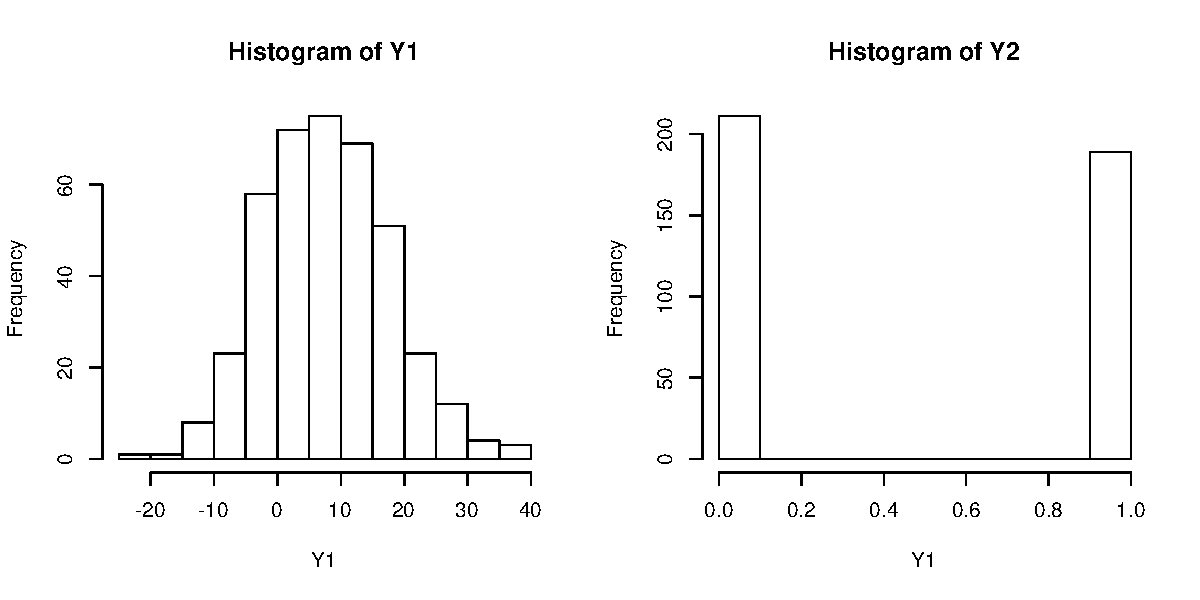
\includegraphics[scale=0.8]{./pic/fig1_histY.pdf}
    \caption{Empirical Distributions of \m{Y1} and \m{Y2}}
 	\label{histY}
\end{figure}

\begin{figure}[!ht]
    \centering
	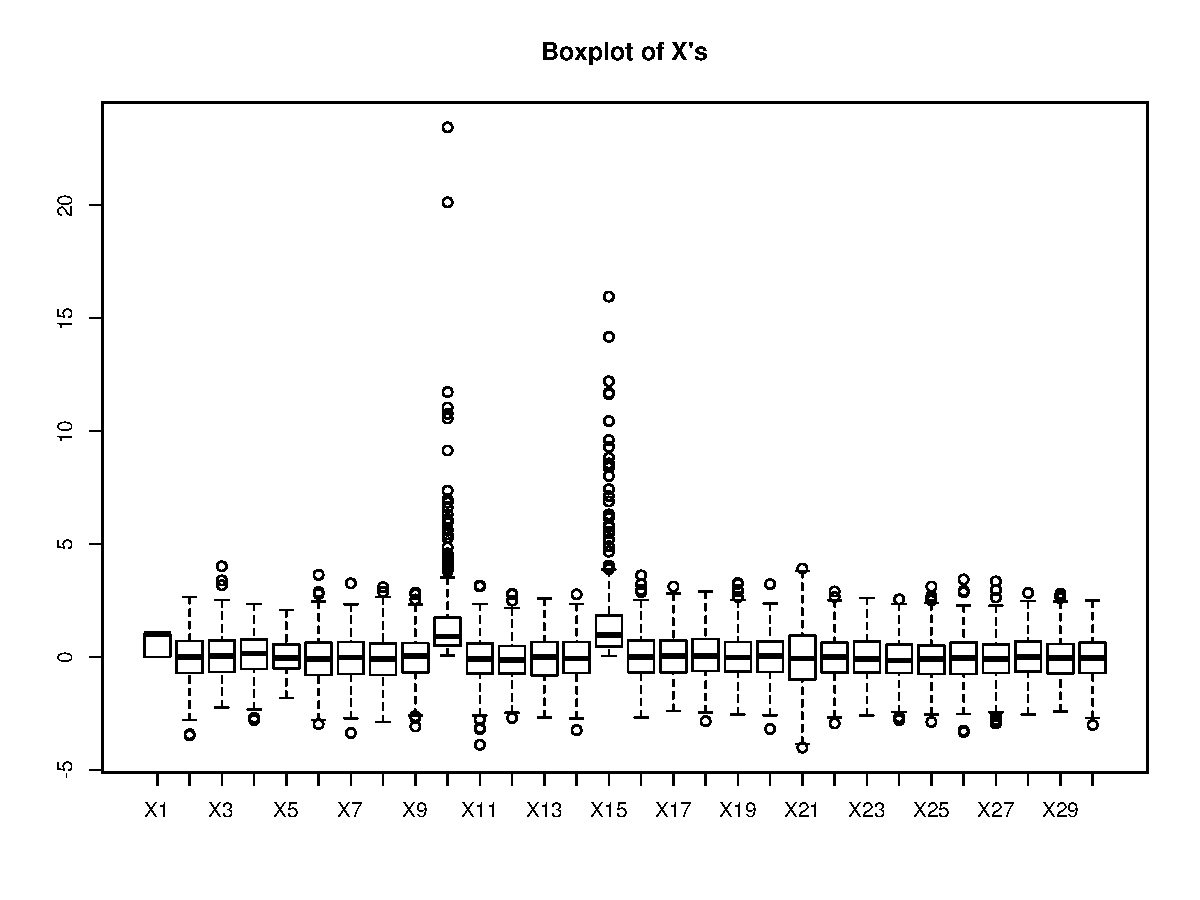
\includegraphics[scale=0.8]{./pic/fig2_boxplot.pdf}
    \caption{Empirical Distributions from \m{X1} to \m{X30}}
 	\label{boxX}
\end{figure}

\begin{figure}[!ht]
    \centering
	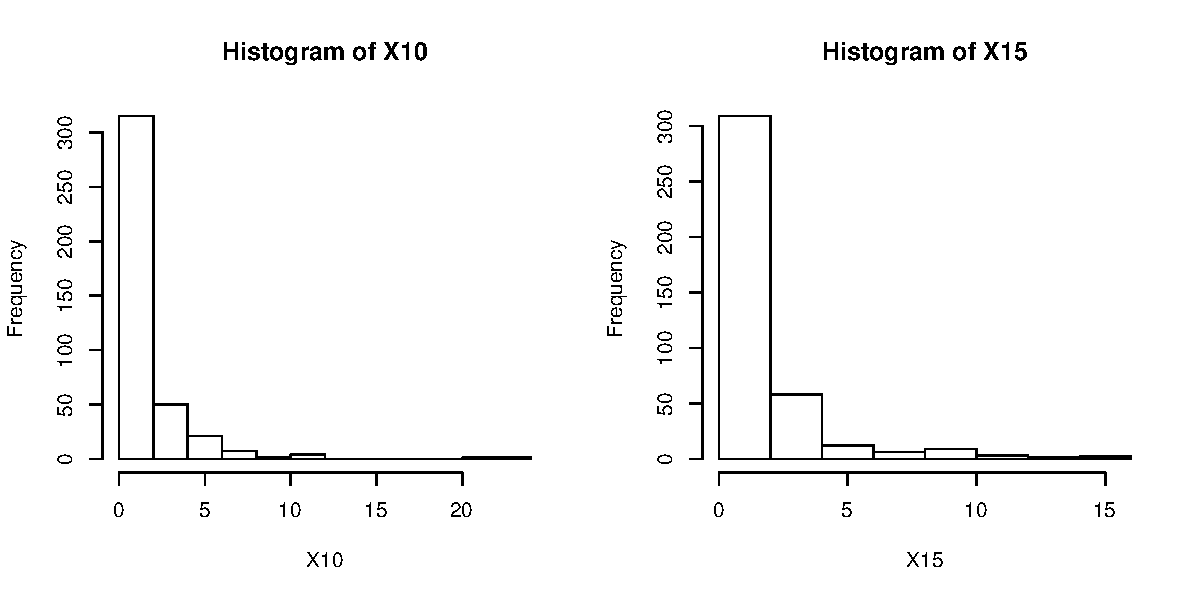
\includegraphics[scale=0.8]{./pic/fig3_histX10X15.pdf}
    \caption{Empirical Distributions of \m{X10} and \m{X15}}
 	\label{distX10X15}
\end{figure}

\begin{figure}[!ht]
    \centering
	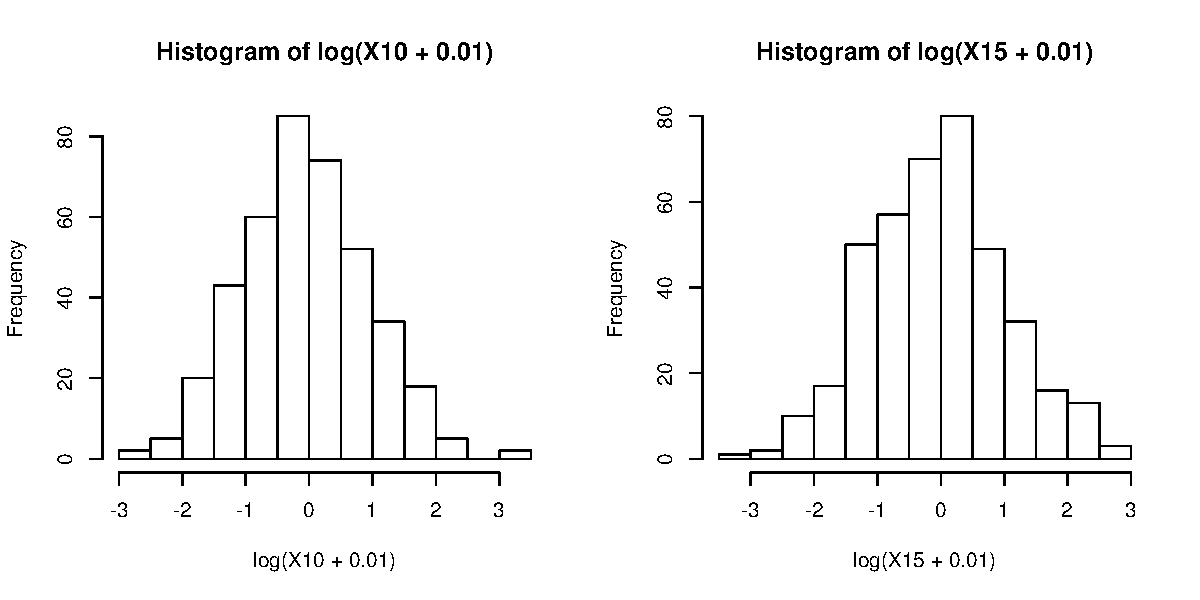
\includegraphics[scale=0.8]{./pic/fig4_histX10X15_trans.pdf}
    \caption{Empirical Distributions of transformed \m{X10} and \m{X15}}
 	\label{distX10X15_trans}
\end{figure}

\begin{landscape}
\begin{figure}[!ht]
    \centering
	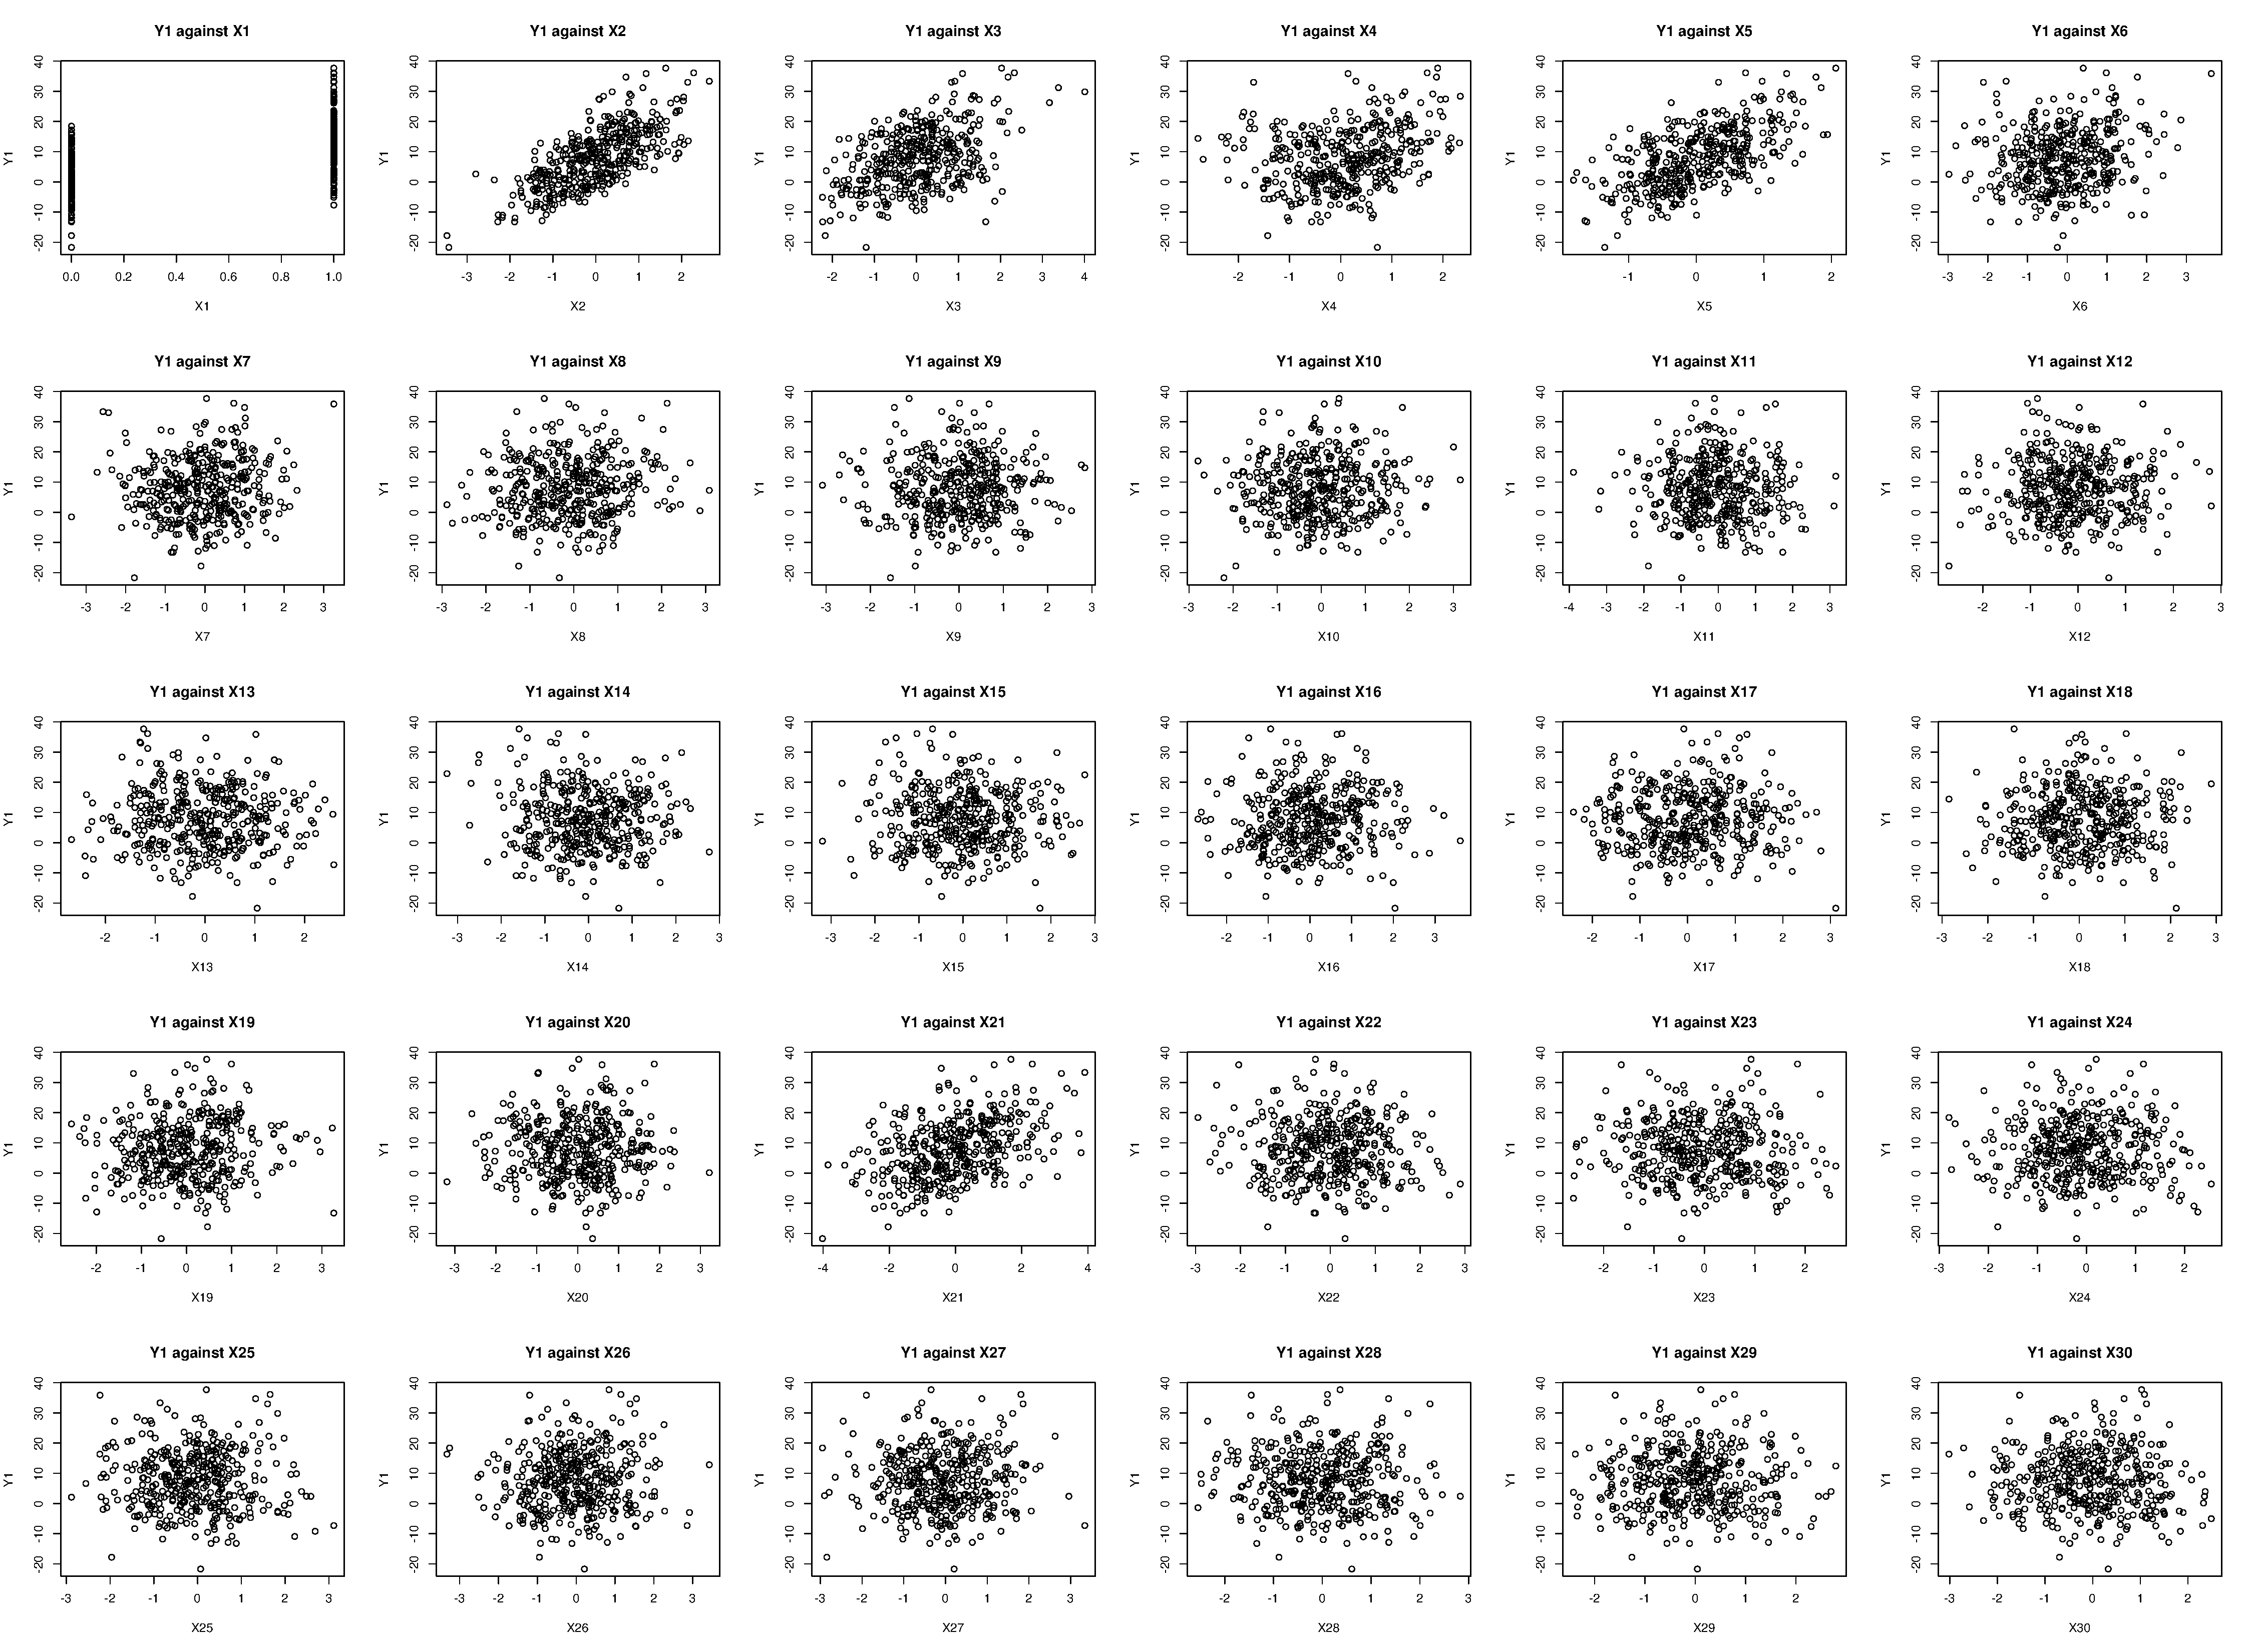
\includegraphics[scale=0.3]{./pic/fig5_scatterPlot.pdf}
    \caption{Scatter-plot for \m{Y1} against \m{X1} to \m{X30}}
 	\label{scatterY1}
\end{figure}

\end{landscape}

\begin{figure}[!ht]
    \centering
	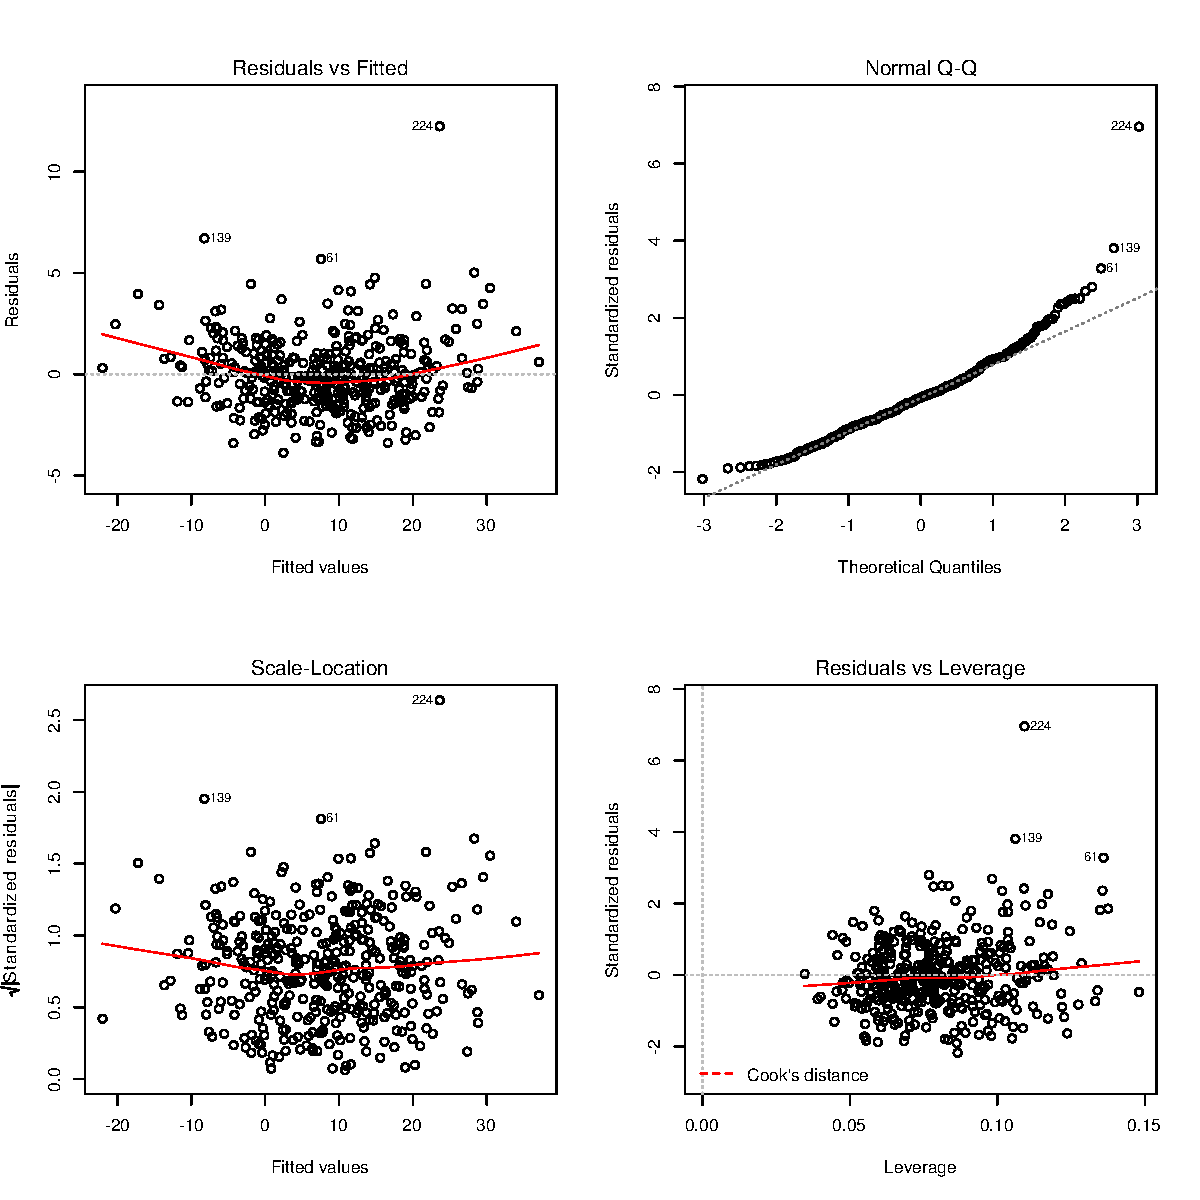
\includegraphics[scale=0.8]{./pic/reg_reg0.pdf}
    \caption{Diagnostic Analysis on reg0}
 	\label{Diagreg0}
\end{figure}

\begin{figure}[!ht]
    \centering
	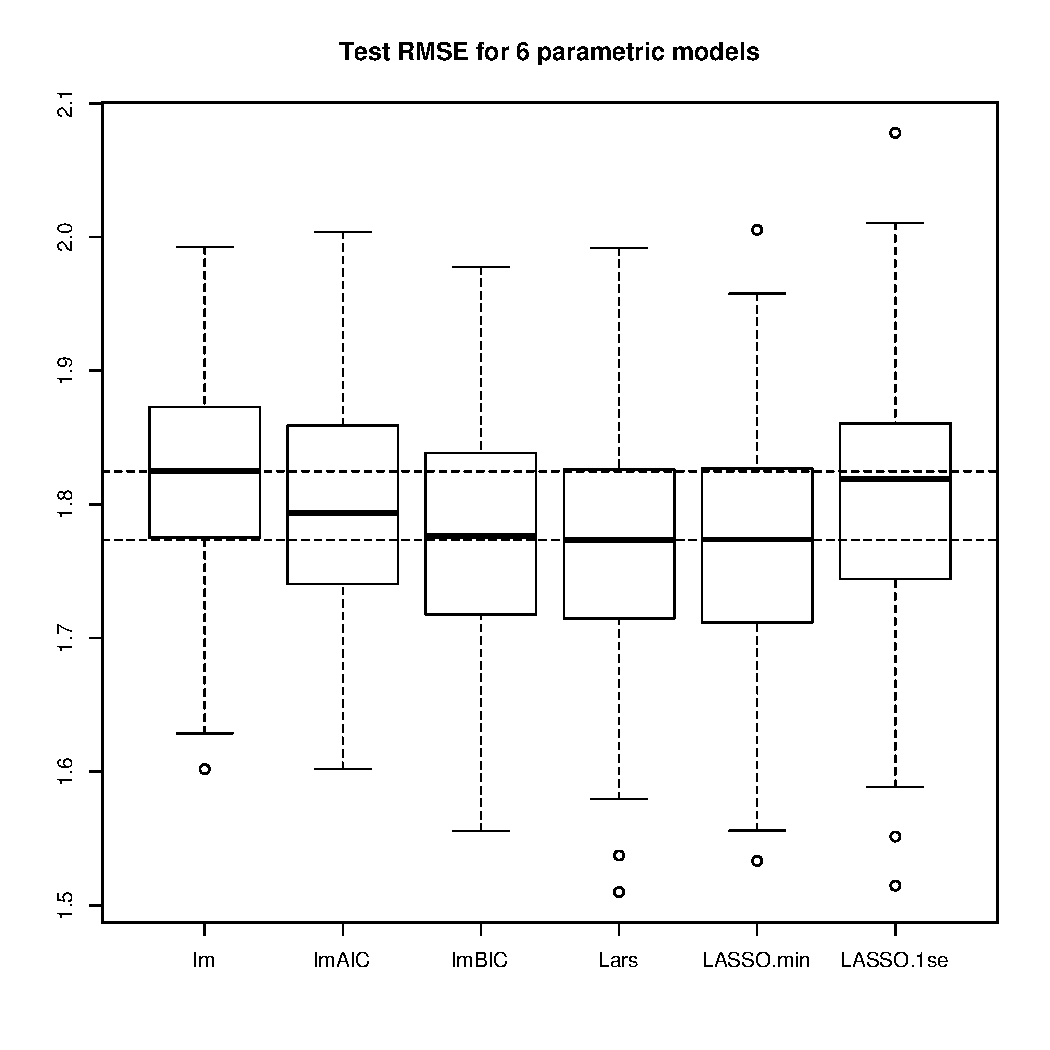
\includegraphics[scale=0.8]{./pic/reg_rmse6.pdf}
    \caption{RMSE of 6 parametric models for Y1}
 	\label{rmse6}
\end{figure}

\begin{figure}[!ht]
    \centering
	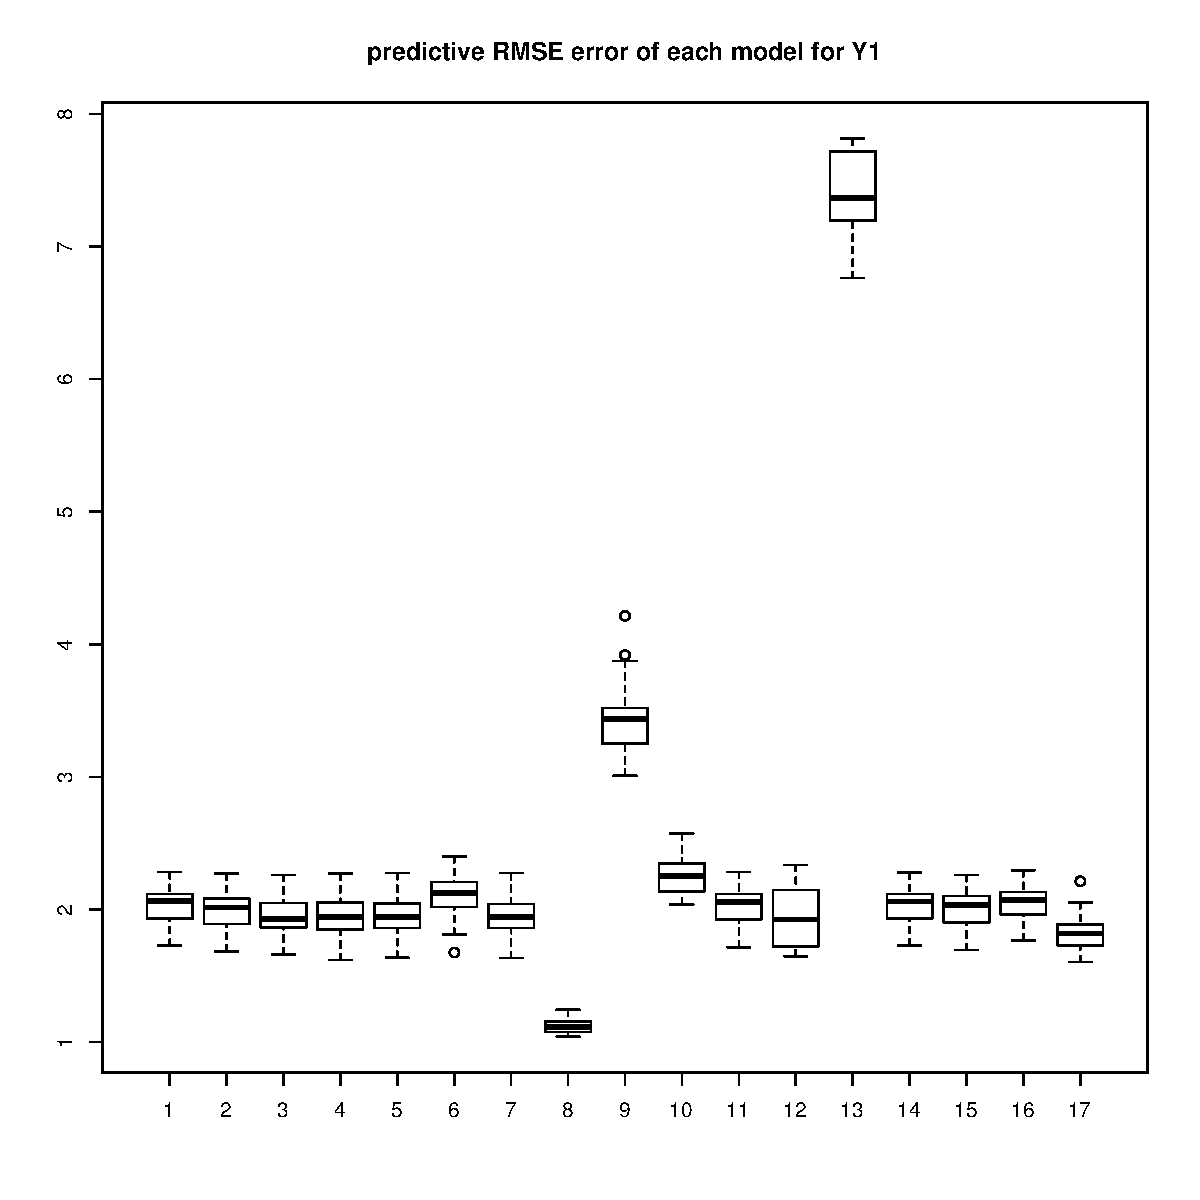
\includegraphics[scale=0.8]{./pic/reg_prediction.pdf}
    \caption{RMSE of predictive models for Y1}
 	\label{rmsep}
\end{figure}

\begin{landscape}
\begin{figure}[!ht]
    \centering
	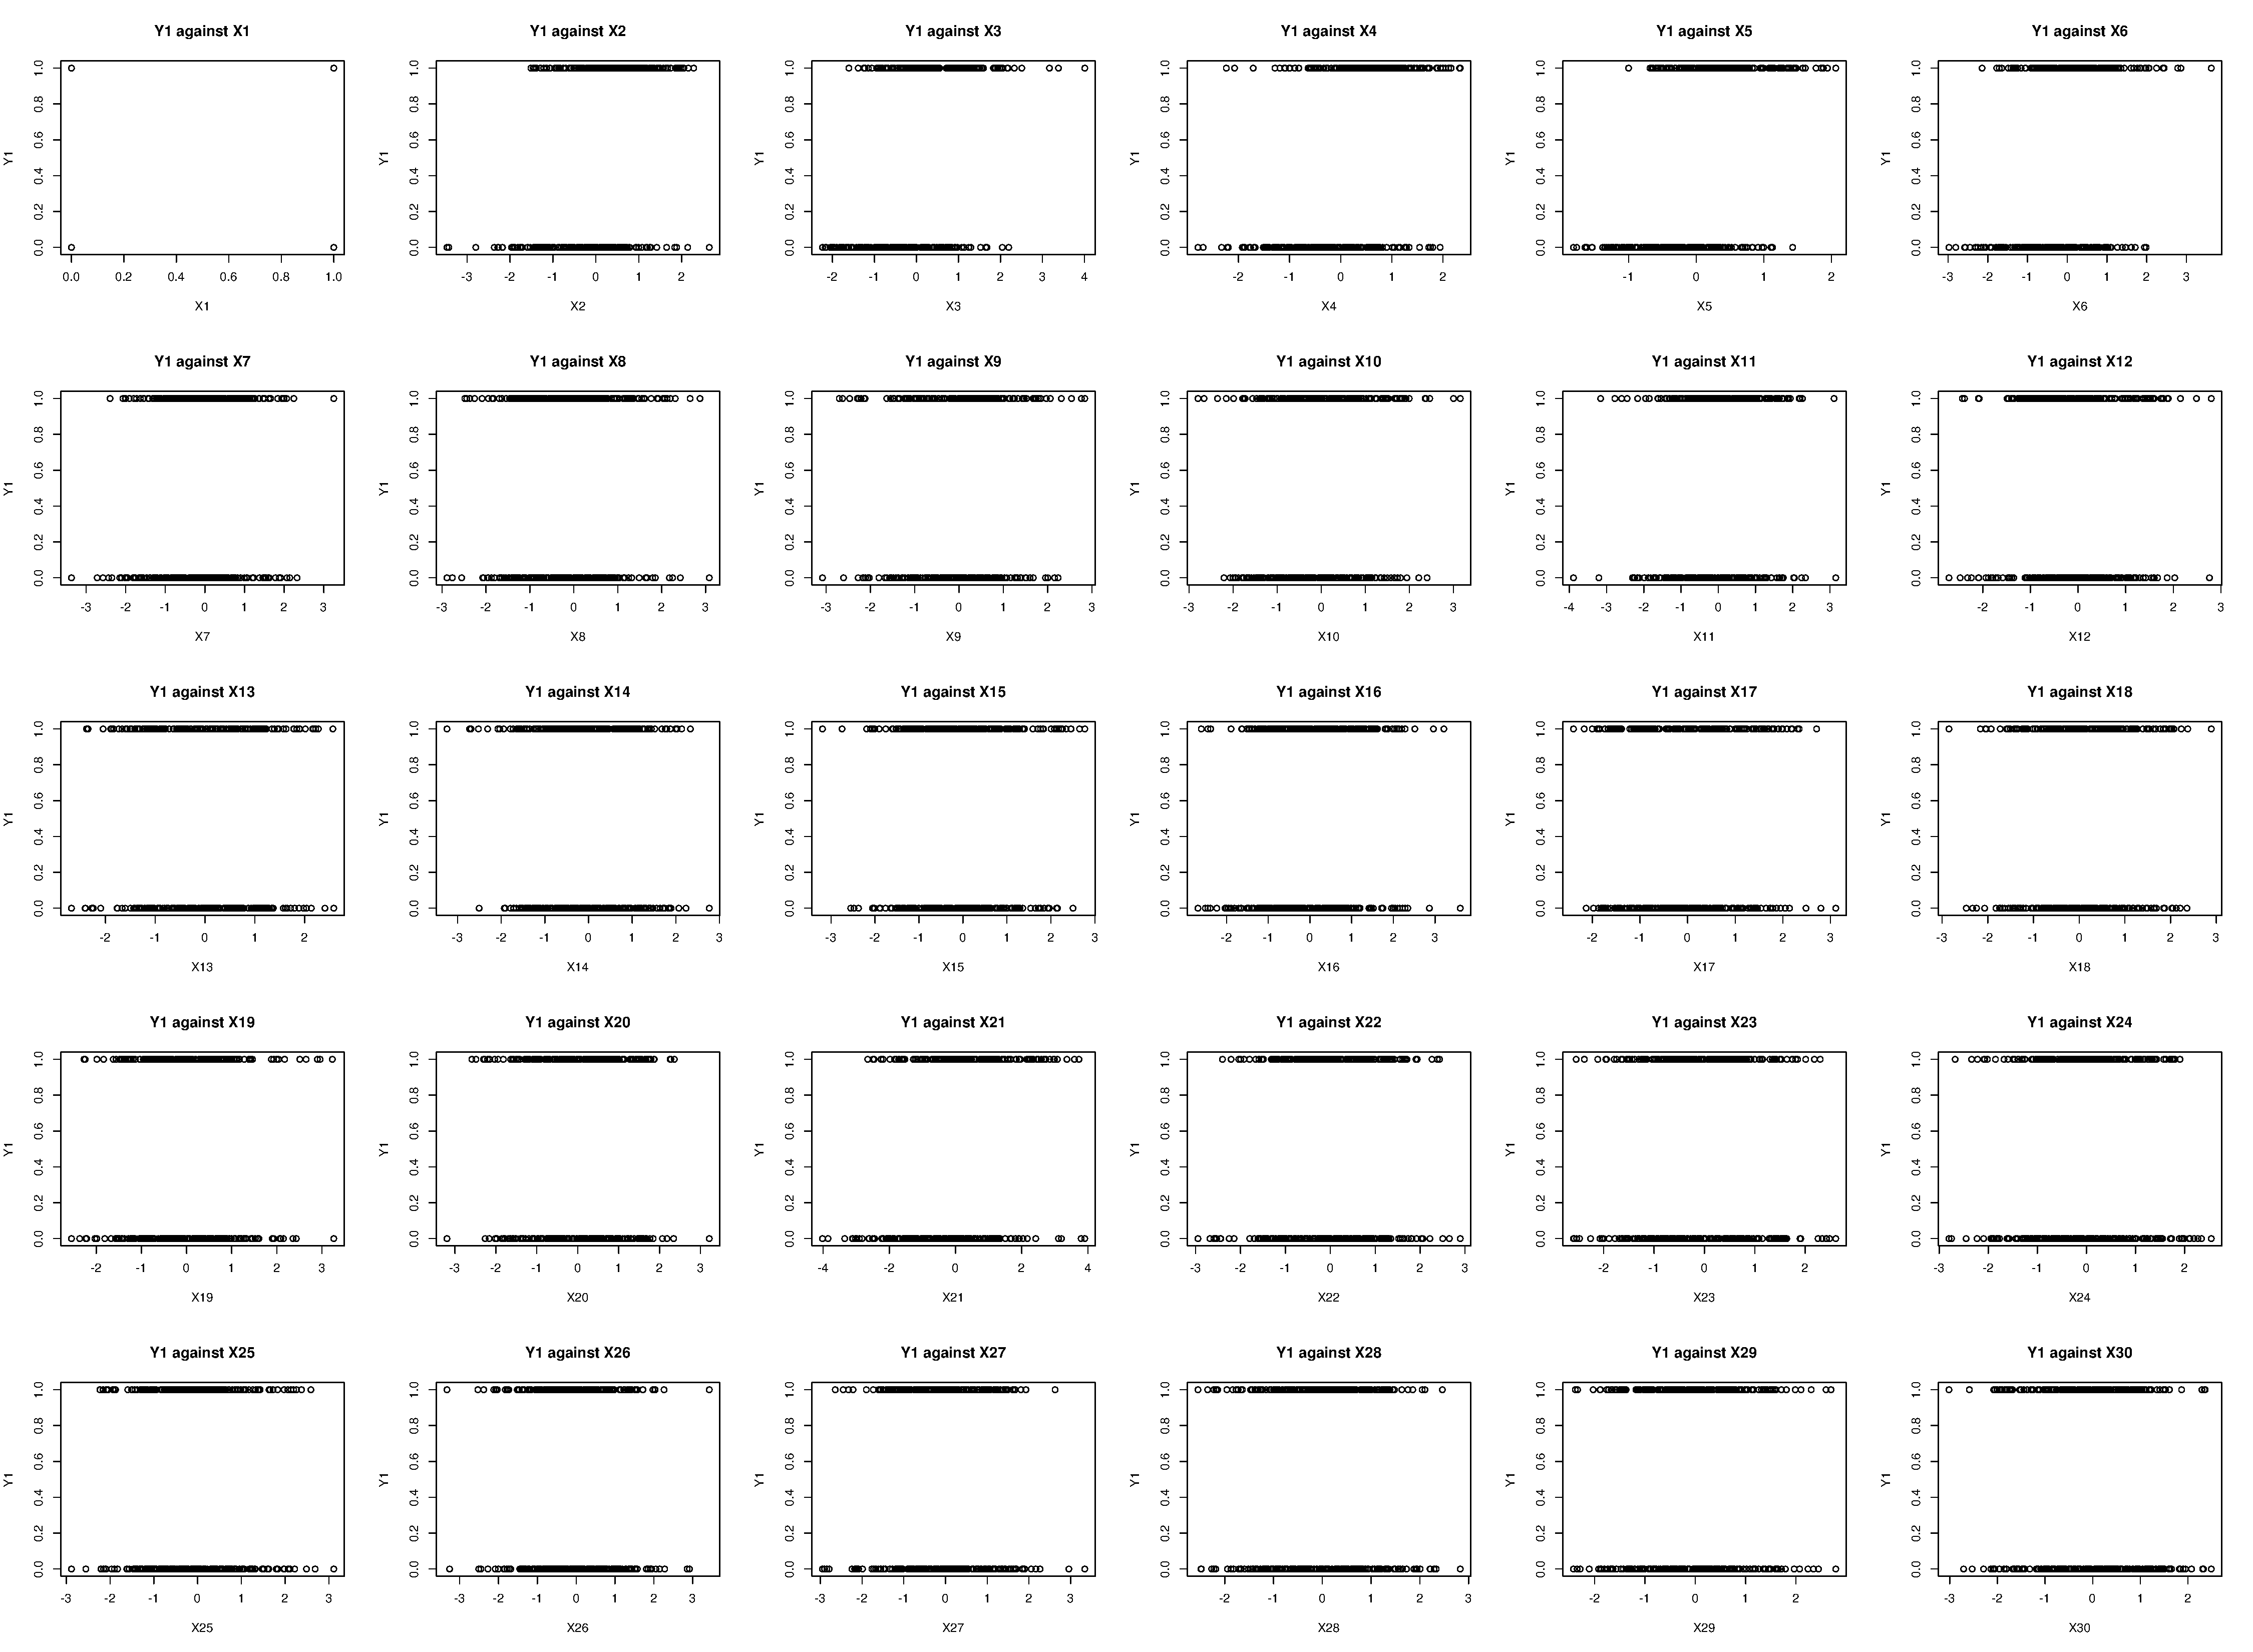
\includegraphics[scale=0.3]{./pic/class_scatterPlot.pdf}
    \caption{Scatter-plot for \m{Y2} against \m{X1} to \m{X30}}
 	\label{scatterY2}
\end{figure}
\end{landscape}

\begin{landscape}
\begin{figure}[!ht]
    \centering
	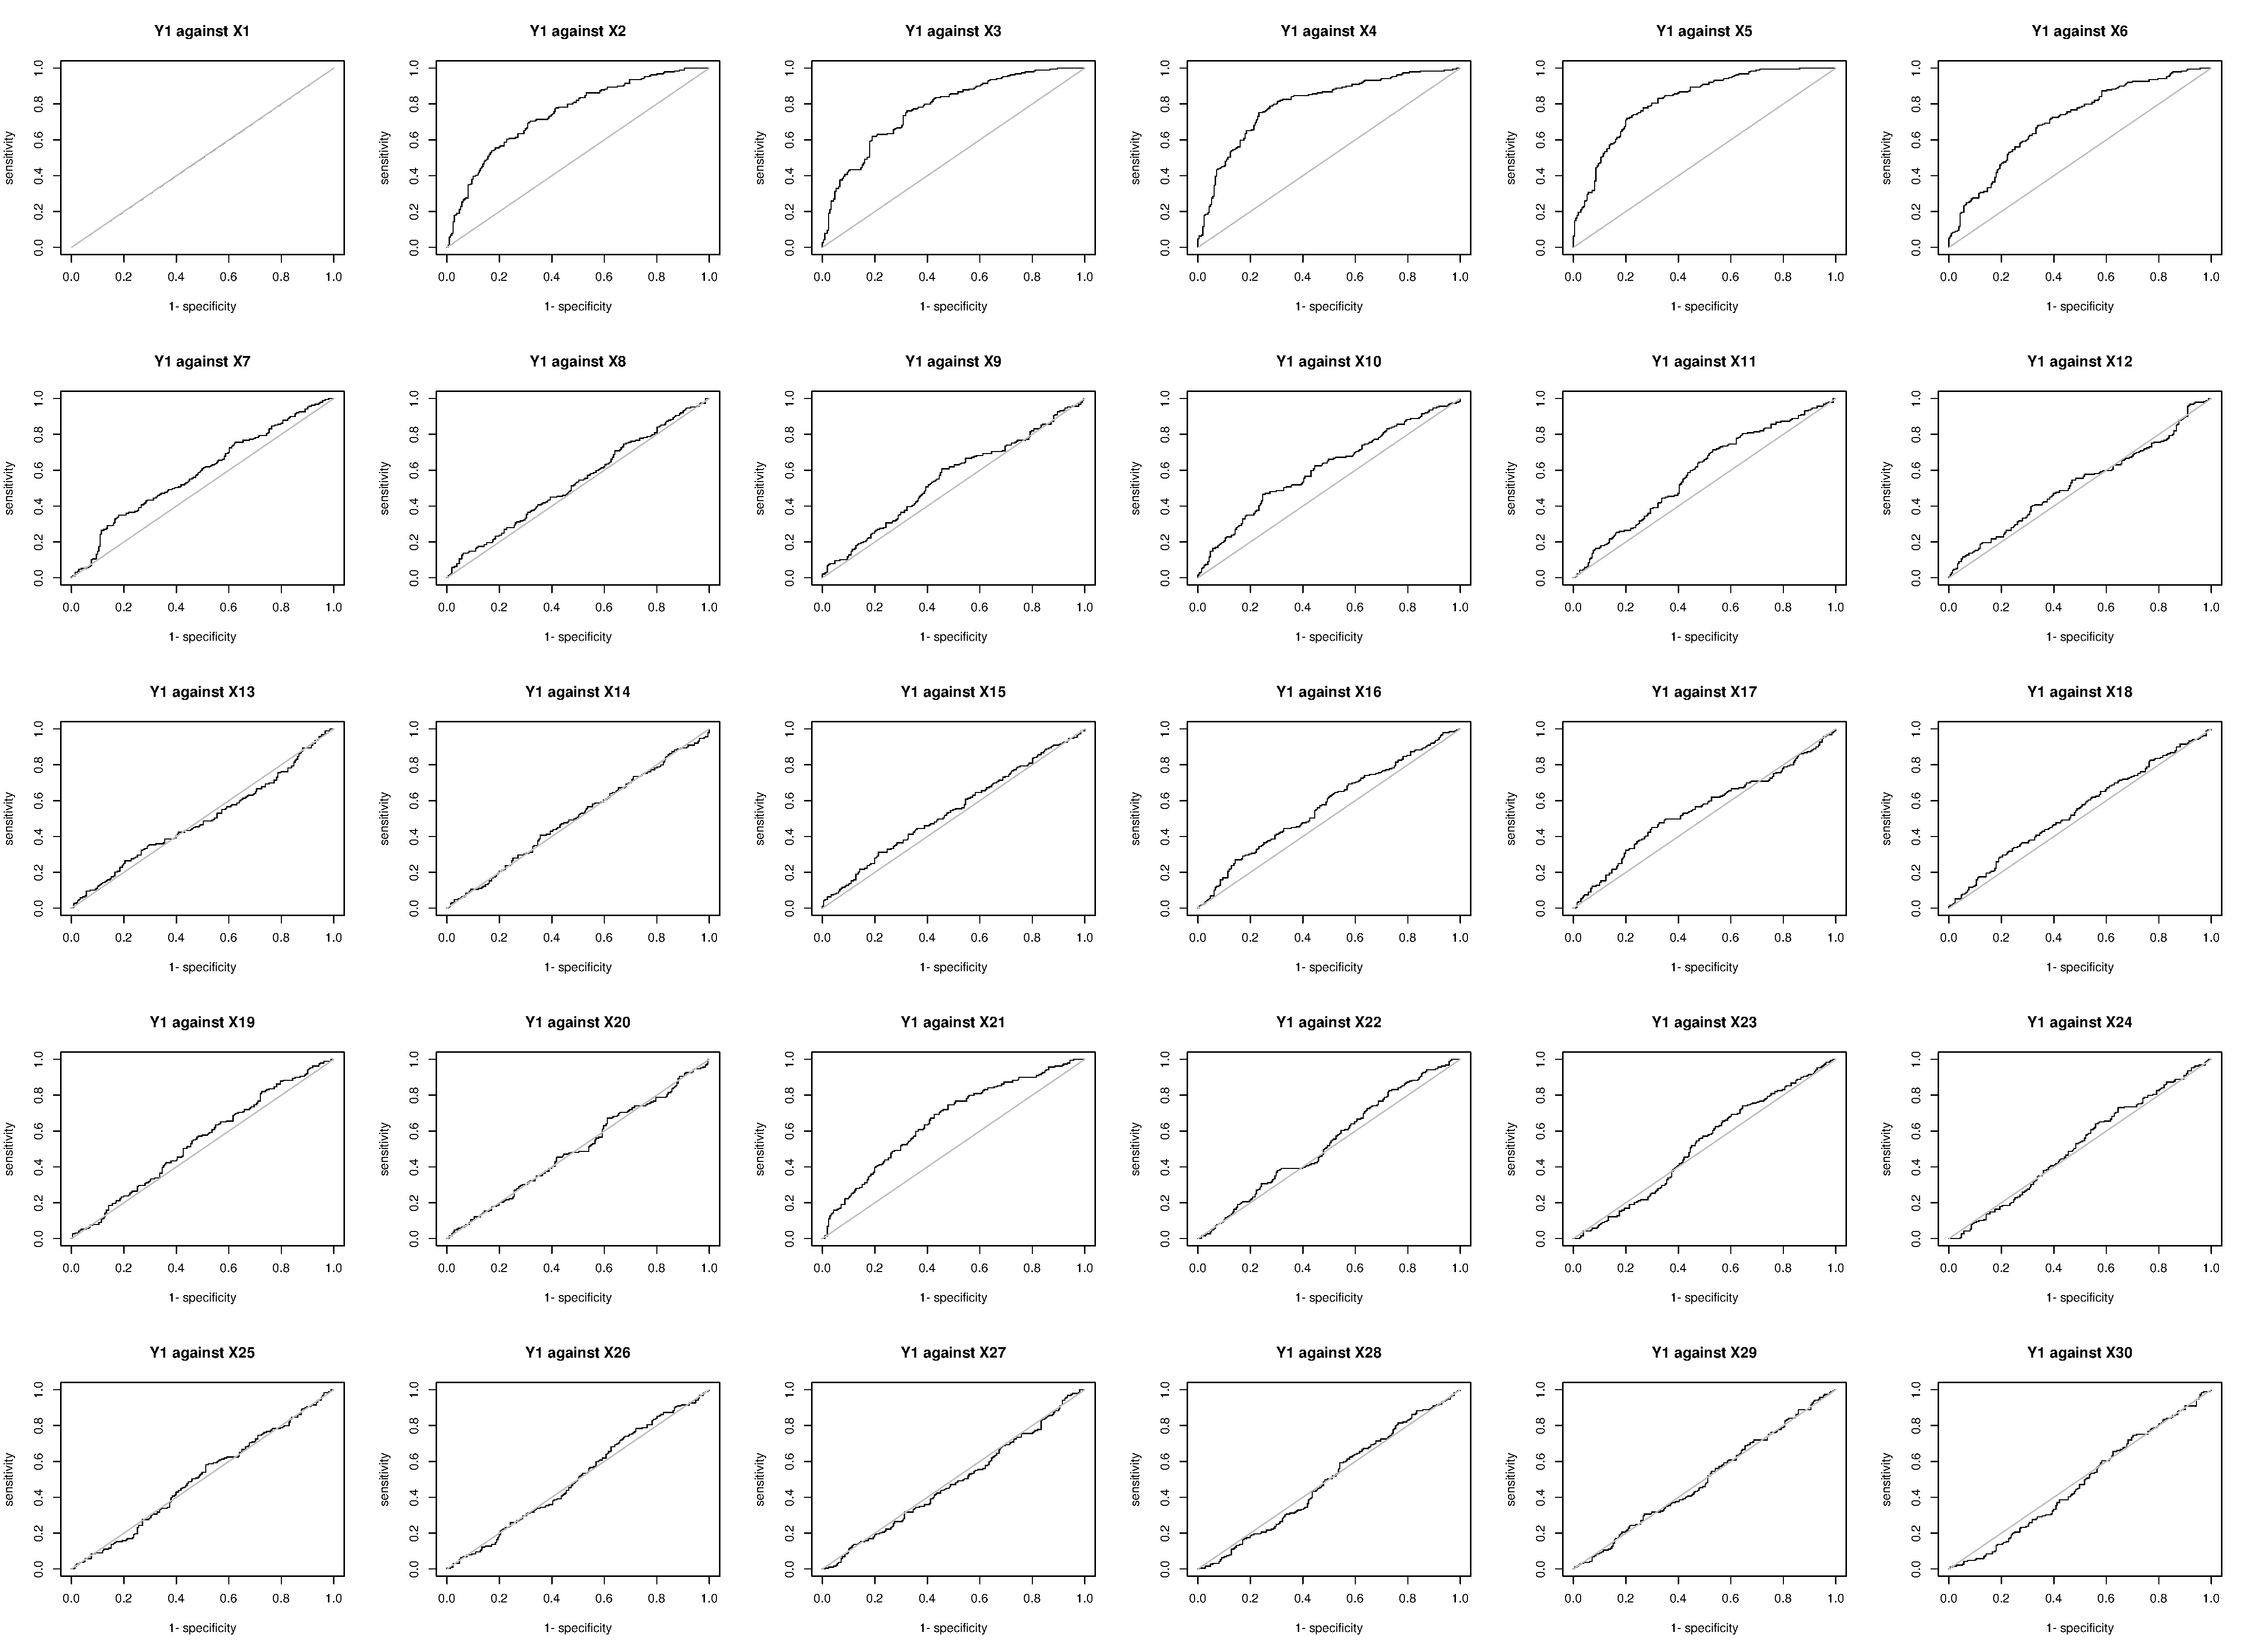
\includegraphics[scale=0.3]{./pic/class_AUCPlot.pdf}
    \caption{Scatter-plot for \m{Y2} against \m{X1} to \m{X30}}
 	\label{rocY2}
\end{figure}
\end{landscape}

\begin{figure}[!ht]
    \centering
	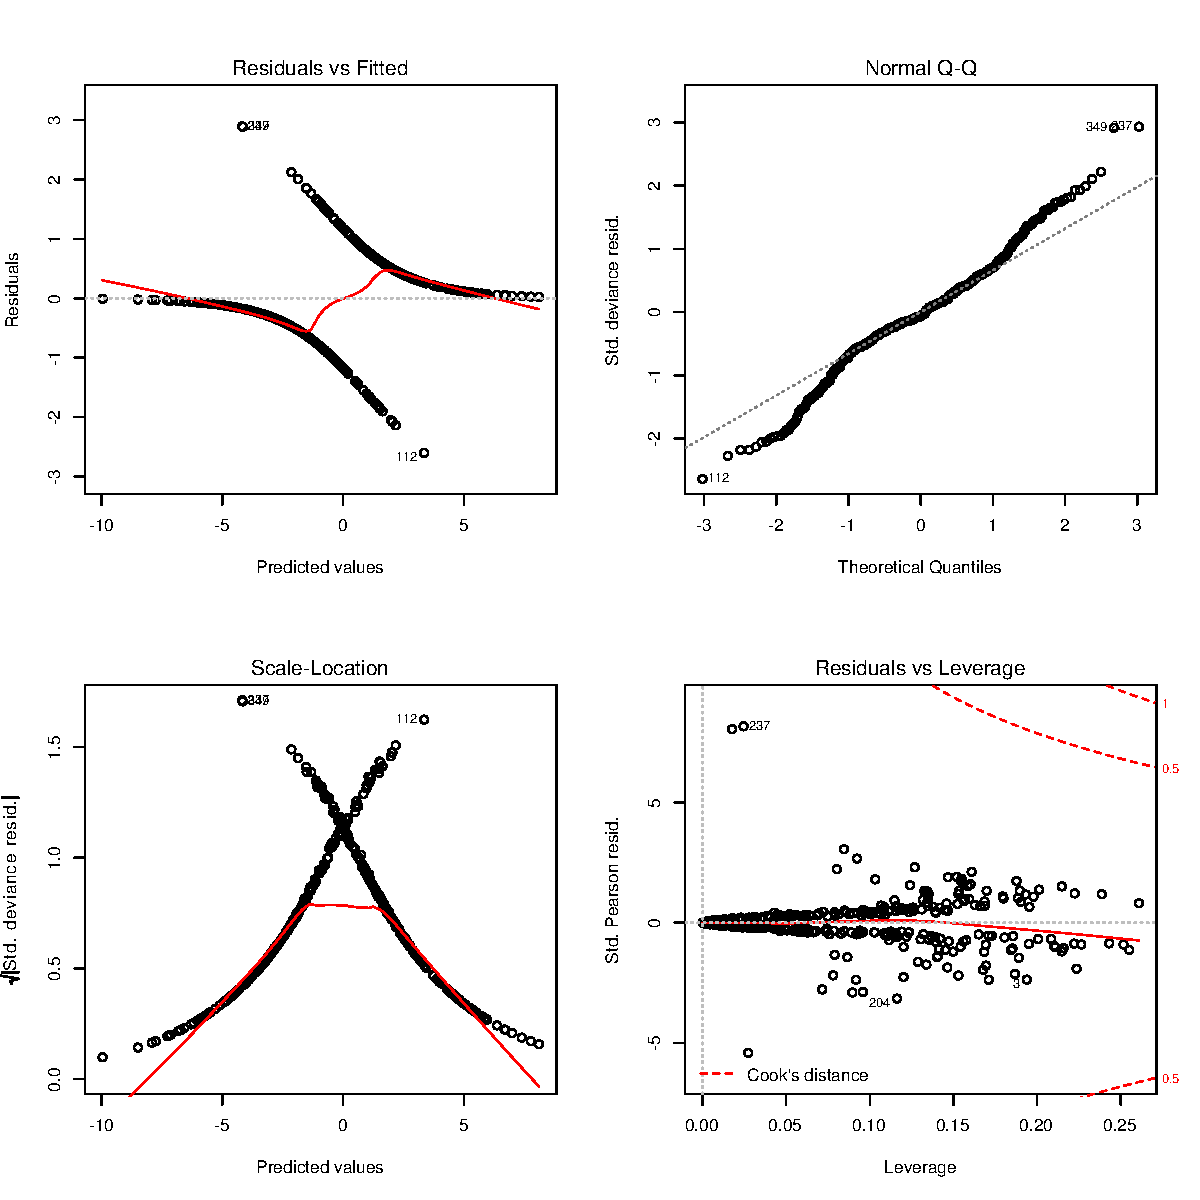
\includegraphics[scale=0.8]{./pic/class_reg0.pdf}
    \caption{Diagnostic Analysis on reg0 for \m{Y2}}
 	\label{DiagregY20}
\end{figure}

\begin{figure}[!ht]
    \centering
	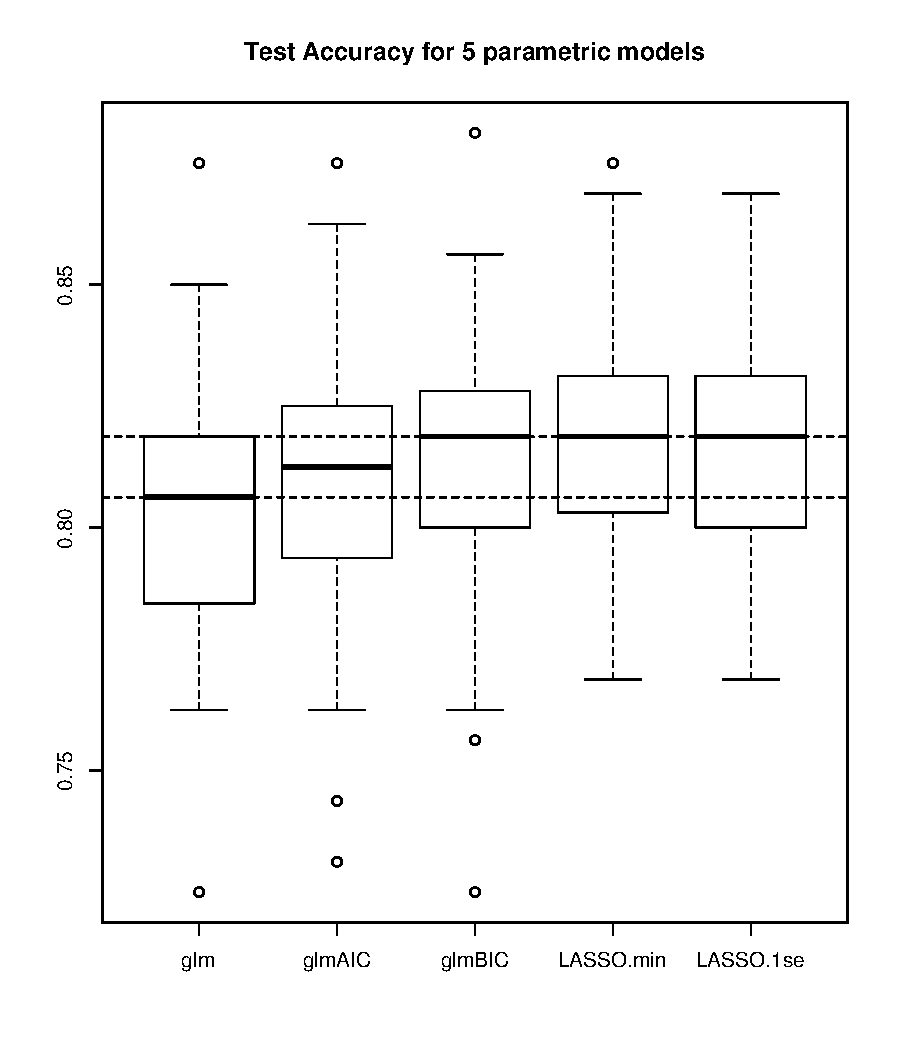
\includegraphics[scale=0.8]{./pic/class_Acc5.pdf}
    \caption{Accuracy of 5 parametric models for Y2}
 	\label{class_acc5}
\end{figure}

\begin{figure}[!ht]
    \centering
	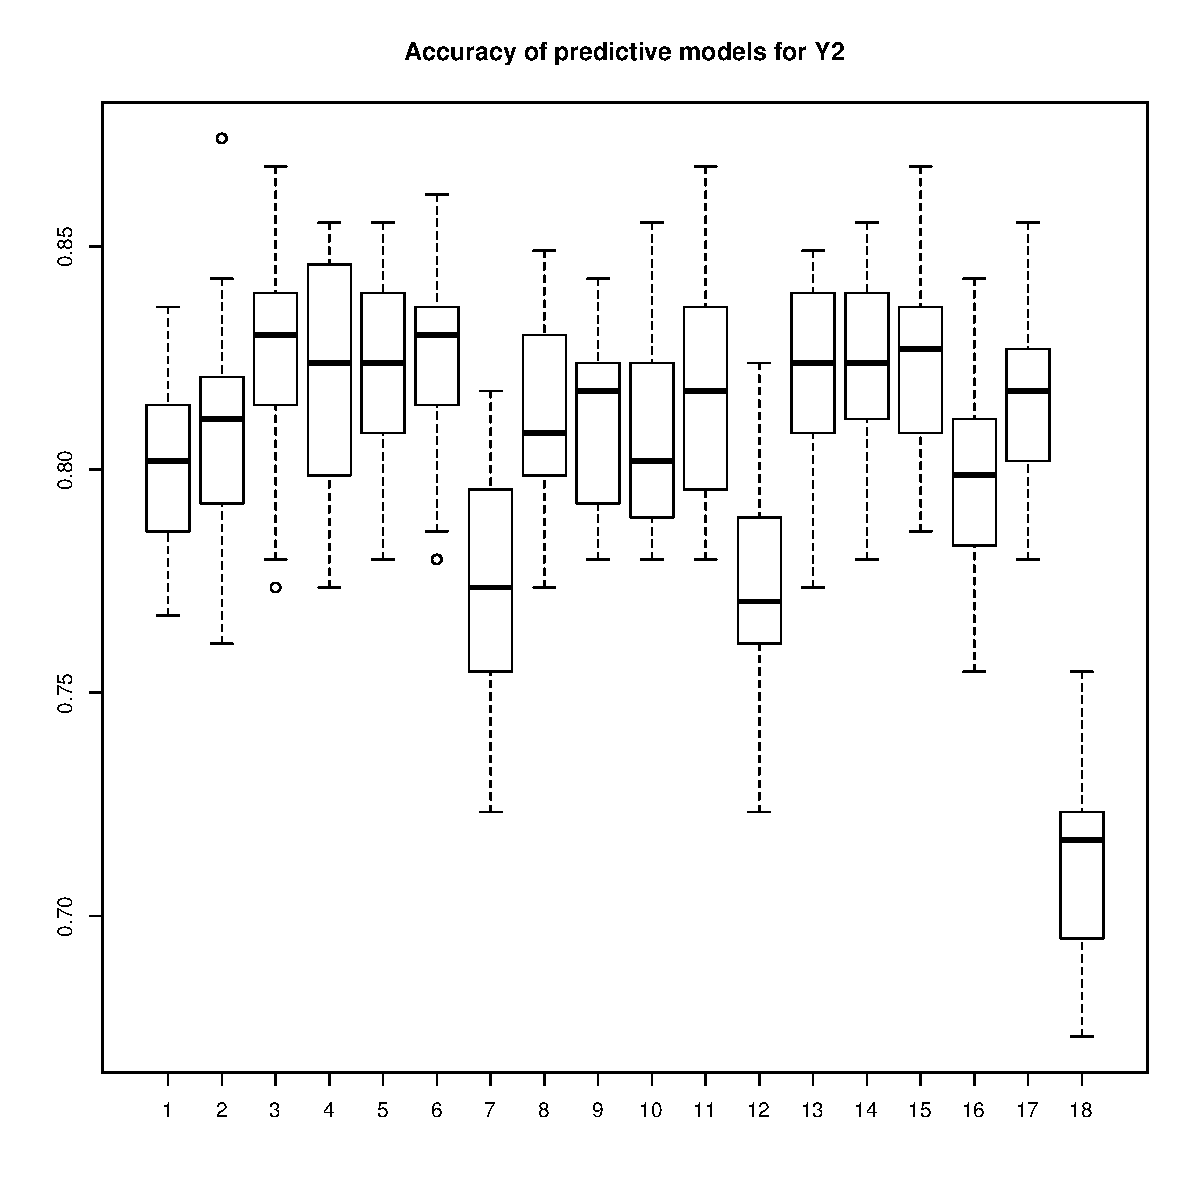
\includegraphics[scale=0.8]{./pic/class_prediction.pdf}
    \caption{Accuracy of predictive models for Y2}
 	\label{accy2}
\end{figure}



\clearpage
\begin{verbatim}
rm(list = ls())


# read data ---------------------------------------------------------------


load("./FinalProject/data.Rda")
load("./FinalProject/pdata.Rda")

picFile <- c("./FinalProject/pic/")
texFile <- c("./FinalProject/tex/")


# preprocessing -----------------------------------------------------------


## distribution of two responses, Histogram
cairo_pdf(filename = paste(picFile, "fig1_histY.pdf", sep = ""), 
          width = 8, height = 4, pointsize = 10)
    par(mfrow = c(1, 2))
    hist(data$Y1, main = "Histogram of Y1", xlab = "Y1")
    hist(data$Y2, main = "Histogram of Y2", xlab = "Y1")
dev.off()

## BoxPlot of predictors
cairo_pdf(filename = paste(picFile, "fig2_boxplot.pdf", sep = ""), 
          width = 8, height = 6, pointsize = 10)
    boxplot(data[, 1:30], main = "Boxplot of X's")
dev.off()

## Distribution of X10 and X15
cairo_pdf(filename = paste(picFile, "fig3_histX10X15.pdf", sep = ""), 
          width = 8, height = 4, pointsize = 10)
    par(mfrow = c(1, 2))
    hist(data$X10, main = "Histogram of X10", xlab = "X10")
    hist(data$X15, main = "Histogram of X15", xlab = "X15")
dev.off()

## Tansform X10 and X15
data$X10 <- log(data$X10 + 0.01)
data$X15 <- log(data$X15 + 0.01)
pdata$X10 <- log(pdata$X10 + 0.01)
pdata$X15 <- log(pdata$X15 + 0.01)

cairo_pdf(filename = paste(picFile, "fig4_histX10X15_trans.pdf", sep = ""), 
          width = 8, height = 4, pointsize = 10)
    par(mfrow = c(1, 2))
    hist(data$X10, main = "Histogram of log(X10 + 0.01)", xlab = "log(X10 + 0.01)")
    hist(data$X15, main = "Histogram of log(X15 + 0.01)", xlab = "log(X15 + 0.01)")
dev.off()


# parametric regression part ----------------------------------------------


## ScatterPlot
cairo_pdf(filename = paste(picFile, "fig5_scatterPlot.pdf", sep = ""), 
          width = 30, height = 22, pointsize = 18)
    par(mfrow = c(5, 6))
    for (i in 1:30) plot(data[, i], data$Y1, 
                         xlab = colnames(data)[i], ylab = "Y1", 
                         main = paste("Y1 against", colnames(data)[i]))
dev.off()

## Include X4^2 into the regression model
data$X4sq <- data$X4^2
pdata$X4sq <- pdata$X4^2

## Base model, multivariate linear regression, reg0
require(car)
reg0 <- lm(Y1 ~ . - Y2, data = data)

cairo_pdf(filename = paste(picFile, "reg_reg0.pdf", sep = ""), 
          width = 8, height = 8, pointsize = 10)
    par(mfrow = c(2, 2))
    plot(reg0)
dev.off()

## Remove outlier, reg1
tmp <- outlierTest(reg0)
outlierIndex <- as.numeric(row.names(as.matrix(tmp$rstudent)))
reg1 <- lm(Y1 ~ . - Y2, data = data, subset = -outlierIndex)

cairo_pdf(filename = paste(picFile, "reg_reg1.pdf", sep = ""), 
          width = 8, height = 8, pointsize = 10)
    par(mfrow = c(2, 2))
    plot(reg1)
dev.off()

ncvTest(reg1)

## Remove redundant predictors by using AIC and BIC regAIC regBIC
regNull <- lm(Y1 ~ 1, data = data, subset = -outlierIndex)

regAIC <- step(reg1, scope = list(lower = regNull, upper = reg1), 
     direction = "both", trace = FALSE)
ncvTest(regAIC)
cairo_pdf(filename = paste(picFile, "reg_regAIC.pdf", sep = ""), 
          width = 8, height = 8, pointsize = 10)
    par(mfrow = c(2, 2))
    plot(regAIC)
dev.off()

regBIC <- step(reg1, scope = list(lower = regNull, upper = reg1), 
              direction = "both", trace = FALSE, k = log(nrow(reg1$model)))
ncvTest(regBIC)
cairo_pdf(filename = paste(picFile, "reg_regBIC.pdf", sep = ""), 
          width = 8, height = 8, pointsize = 10)
    par(mfrow = c(2, 2))
    plot(regBIC)
dev.off()


# 
# texreg(l = list(reg0, reg1, regAIC, regBIC), single.row = T,
#        leading.zero = FALSE, booktabs = TRUE, dcolumn = TRUE)


## Feature Selection using LASSO, lambda tuned by CV
require(glmnet)
X <- as.matrix(data[-outlierIndex, c(1:30, 33)])
y <- as.matrix(data$Y1[-outlierIndex])

regLASSOcv <- cv.glmnet(X, y, nfolds = 10)
# plot(regLASSOcv)

regLASSO_1 <- glmnet(X, y, lambda = regLASSOcv$lambda.min)
regLASSO_2 <- glmnet(X, y, lambda = regLASSOcv$lambda.1se)

cairo_pdf(filename = paste(picFile, "reg_regLASSO.pdf", sep = ""), 
          width = 8, height = 4, pointsize = 10)
    par(mfrow = c(1, 2))
    qqnorm(predict(regLASSO_1, X))
    qqline(y, col = 2)
    qqnorm(predict(regLASSO_2, X))
    qqline(y, col = 2)
dev.off()


## Feature selection using lars, lambda selected by smallest Cp statistic
require(lars)
regLars <- lars(x = X, y = y, type = "lasso")
s <- which.min(summary(regLars)$Cp)
predLars <- predict(regLars, type = "fit", newx = X, s = s, mode = "step")$fit

cairo_pdf(filename = paste(picFile, "reg_regLars.pdf", sep = ""), 
          width = 4, height = 4, pointsize = 10)
    qqnorm(predLars)
    qqline(y, col = 2)
dev.off()

foo <- cbind(as.matrix(coef(regLASSO_1))[2:32], as.matrix(coef(regLASSO_2))[2:32], as.matrix(coef(regLars)[s, ]))
foo <- round(foo, 2)
write.table(foo, "./FinalProject/reglasso")



# prediction power --------------------------------------------------------


## Selection from lm, lmAIC, lmBIC, LASSO by outer cross-validation
require(caret)
require(doMC)
registerDoMC(2)

fitControl <- trainControl(## 10-fold CV
    method = "repeatedcv",
    number = 10, 
    repeats = 1
)

fitControl0 <- trainControl(## 10-fold CV
    method = "none",
)

num_iter = 40
result <- matrix(nrow = num_iter, ncol = 6)
data0 <- data[-outlierIndex, ]
set.seed(123)

for (jj in 1:num_iter)
{
    i = 1
    trainIndex <- createDataPartition(data0$Y1, p = .6,
                                      list = FALSE,
                                      times = 1)
    data_train <- data0[trainIndex, ]
    data_test <- data0[-trainIndex, ]
    
    ## regression part
    X_train <- data_train[, c(1:30, 33)]
    y_train <- data_train[, 31]
    X_test <- data_test[, c(1:30, 33)]
    y_test <- data_test[, 31]
    
    ## simple linear regression
    m <- train(y = y_train, x = X_train,
               trControl = fitControl0,
               method = "lm")
    result[jj, i] <- sqrt(mean((y_test - predict(m, newdata = X_test))^2))
    i = i + 1
    
    ## stepwise linear model AIC
    m <- train(y = y_train, x = X_train,
               trControl = fitControl0,
               method = "lmStepAIC", trace = FALSE)
    result[jj, i] <- sqrt(mean((y_test - predict(m, newdata = X_test))^2))
    i = i + 1
    
    ## stepwise linear model BIC
    m <- train(y = y_train, x = X_train,
               trControl = fitControl0,
               method = "lmStepAIC", trace = FALSE, 
               k = log(nrow(X_train)))
    result[jj, i] <- sqrt(mean((y_test - predict(m, newdata = X_test))^2))
    i = i + 1
    
    ## lasso (lars)
    m <- train(y = y_train, x = X_train,
               trControl = fitControl,
               method = "lars2", 
               tuneGrid = expand.grid(step = 2:31))
    result[jj, i] <- sqrt(mean((y_test - predict(m, newdata = X_test))^2))
    i = i + 1
    
    ## lasso (glmnet) lambda.min
    m <- train(y = y_train, x = X_train,
               trControl = fitControl,
               method = "glmnet", 
               tuneGrid = expand.grid(alpha = 1, 
                                      lambda = seq(0.001, 0.2, 0.002)))
    result[jj, i] <- sqrt(mean((y_test - predict(m, newdata = X_test))^2))
    i = i + 1
    
    ## lasso (glmnet) lambda.1se
    mcv <- cv.glmnet(as.matrix(X_train), as.matrix(y_train), nfolds = 10, 
                     lambda = seq(0.001, 0.2, 0.002))
    m <- glmnet(as.matrix(X_train), as.matrix(y_train), lambda = mcv$lambda.1se)
    result[jj, i] <- sqrt(mean((y_test - predict(m, as.matrix(X_test)))^2))
    
    print(jj)
}

cairo_pdf(filename = paste(picFile, "reg_rmse6.pdf", sep = ""), 
          width = 7, height = 7, pointsize = 10)
    boxplot(result, main = "Test RMSE for 6 parametric models",
            names = c("lm", "lmAIC", "lmBIC", "Lars", "LASSO.min", "LASSO.1se"))
    abline(median(result[,1]), 0, lty = 2)
    abline(min(apply(result, 2, median)), 0, lty = 2)
dev.off()

##write.table(result, file = "./FinalProject/regResultPara")
\end{verbatim}

\clearpage
\begin{verbatim}
rm(list = ls())

data1 <- read.table(file = "./FinalProject/data/data1")
data2 <- read.table(file = "./FinalProject/data/data2")
data3 <- read.table(file = "./FinalProject/data/data3")

pdata1 <- read.table(file = "./FinalProject/data/pdata1")
pdata2 <- read.table(file = "./FinalProject/data/pdata2")

data <- data.frame(data1, data2, data3)
pdata <- data.frame(pdata1, pdata2)
## X1 - X30 are predictors, where X1 is {0, 1} and others are continuous
## Y1 - Y2 are responses, where Y1 is continous and Y2 is {0, 1}
##data <- data[, 1:31]
data$X10 <- log(data$X10 + 0.01)
data$X15 <- log(data$X15 + 0.01)
data$X4sq <- data$X4 ^ 2

pdata$X10 <- log(pdata$X10 + 0.01)
pdata$X15 <- log(pdata$X15 + 0.01)
pdata$X4sq <- pdata$X4 ^ 2


require(doMC)
registerDoMC(2)
require(caret)

set.seed(9876)

fitControl <- trainControl(## 10-fold CV
    method = "repeatedcv",
    number = 10, 
    repeats = 1
)

fitControl_tree <- trainControl(## OOB
    method = "oob"
)


num_iter = 20
result <- matrix(nrow = 18, ncol = num_iter)


for (jj in 1:num_iter)
{
    trainIndex <- createDataPartition(data$Y1, p = .6,
                                      list = FALSE,
                                      times = 1)
    data_train <- data[trainIndex, ]
    data_test <- data[-trainIndex, ]
    
    ## regression part
    X_train <- data_train[, c(1:30, 33)]
    y_train <- data_train[, 31]
    X_test <- data_test[, c(1:30, 33)]
    y_test <- data_test[, 31]
    stacking <- matrix(nrow = nrow(X_train), ncol = 20)
    stacking_test <- matrix(nrow = nrow(X_test), ncol = 20)
    i = 1
    
    
    ## simple linear model, lm, 2.115021
    m <- train(y = y_train, x = X_train,
               trControl = fitControl,
               method = "lm")
    result[i, jj] <- sqrt(mean((y_test - predict(m, newdata = X_test))^2))
    stacking[,i] = predict(m)
    stacking_test[,i] = predict(m, newdata = X_test)
    i = i + 1
    
    ## stepwise linear model AIC, 2.089027
    m <- train(y = y_train, x = X_train,
               trControl = fitControl,
               method = "lmStepAIC", trace = FALSE)
    result[i, jj] <- sqrt(mean((y_test - predict(m, newdata = X_test))^2))
    stacking[,i] = predict(m)
    stacking_test[,i] = predict(m, newdata = X_test)
    i = i + 1
    
    ## stepwise linear model BIC, 2.030876
    m <- train(y = y_train, x = X_train,
               trControl = fitControl,
               method = "lmStepAIC", trace = FALSE, 
               k = log(nrow(X_train) * 9 / 10))
    result[i, jj] <- sqrt(mean((y_test - predict(m, newdata = X_test))^2))
    stacking[,i] = predict(m)
    stacking_test[,i] = predict(m, newdata = X_test)
    i = i + 1
    
    ## lasso (lars), 2.046749
    m <- train(y = y_train, x = X_train,
               trControl = fitControl,
               method = "lars2", 
               tuneGrid = expand.grid(step = 2:31))
    result[i, jj] <- sqrt(mean((y_test - predict(m, newdata = X_test))^2))
    stacking[,i] = predict(m)
    stacking_test[,i] = predict(m, newdata = X_test)
    i = i + 1
    
    ## lasso (glmnet) 2.046684
    m <- train(y = y_train, x = X_train,
               trControl = fitControl,
               method = "glmnet", 
               tuneGrid = expand.grid(alpha = 1, 
                                      lambda = seq(0.001, 0.2, 0.002)))
    result[i, jj] <- sqrt(mean((y_test - predict(m, newdata = X_test))^2))
    stacking[,i] = predict(m)
    stacking_test[,i] = predict(m, newdata = X_test)
    i = i + 1
    
    ## ridge (glmnet) 2.206863
    m <- train(y = y_train, x = X_train,
               trControl = fitControl,
               method = "glmnet", 
               tuneGrid = expand.grid(alpha = 0, 
                                      lambda = seq(0.01, 1, 0.01)))
    result[i, jj] <- sqrt(mean((y_test - predict(m, newdata = X_test))^2))
    stacking[,i] = predict(m)
    stacking_test[,i] = predict(m, newdata = X_test)
    i = i + 1
    
    ## elastic net (glmnet) 2.046684
    m <- train(y = y_train, x = X_train,
               trControl = fitControl,
               method = "glmnet", 
               tuneGrid = expand.grid(alpha = seq(0.7, 1, 0.05), 
                                      lambda = seq(0.001, 0.2, 0.002)))
    result[i, jj] <- sqrt(mean((y_test - predict(m, newdata = X_test))^2))
    stacking[,i] = predict(m)
    stacking_test[,i] = predict(m, newdata = X_test)
    i = i + 1
    
    # mars, best
    m <- train(y = y_train, x = X_train[, 1:30],
               trControl = fitControl,
               method = "gcvEarth", 
               tuneGrid = expand.grid(degree = 1:5))
    result[i, jj] <- sqrt(mean((y_test - predict(m, newdata = X_test))^2))
    stacking[,i] = predict(m)
    stacking_test[,i] = predict(m, newdata = X_test)
    i = i + 1
    
    ## random forest, 3.860662
    m <- train(y = y_train, x = X_train,
               trControl = fitControl_tree,
               method = "rf", 
               tuneGrid = expand.grid(mtry = seq(13, 23, 1)))
    result[i, jj] <- sqrt(mean((y_test - predict(m, newdata = X_test))^2))
    stacking[,i] = predict(m)
    stacking_test[,i] = predict(m, newdata = X_test)
    i = i + 1
    
    ## gradient boosting tree, 2.710811
    m <- train(y = y_train, x = X_train,
               trControl = fitControl,
               method = "gbm", 
               tuneGrid = expand.grid(n.trees = seq(500, 1000, 100), 
                                      shrinkage = 0.05, 
                                      interaction.depth = 1:4), 
               distribution = "gaussian", 
               n.minobsinnode = 5)
    result[i, jj] <- sqrt(mean((y_test - predict(m, newdata = X_test))^2))
    stacking[,i] = predict(m)
    stacking_test[,i] = predict(m, newdata = X_test)
    i = i + 1
    
    ## Gaussian Process with linear kernal, 2.113074
    m <- train(y = y_train, x = X_train,
               trControl = fitControl,
               method = "gaussprLinear")
    result[i, jj] <- sqrt(mean((y_test - predict(m, newdata = X_test))^2))
    stacking[,i] = predict(m)
    stacking_test[,i] = predict(m, newdata = X_test)
    i = i + 1
    
    ## Gaussian Process with Polynomial Kernel, 1.943231
    m <- train(y = y_train, x = X_train,
               trControl = fitControl,
               method = "gaussprPoly")
    result[i, jj] <- sqrt(mean((y_test - predict(m, newdata = X_test))^2))
    stacking[,i] = predict(m)
    stacking_test[,i] = predict(m, newdata = X_test)
    i = i + 1
    
    ## knn, 7.602605
    m <- train(y = y_train, x = X_train,
               trControl = fitControl,
               method = "knn",
               tuneGrid = expand.grid(k = seq(1, 20, 2)))
    result[i, jj] <- sqrt(mean((y_test - predict(m, newdata = X_test))^2))
    stacking[,i] = predict(m)
    stacking_test[,i] = predict(m, newdata = X_test)
    i = i + 1
    
    ## pls, 2.111247
    m <- train(y = y_train, x = X_train,
               trControl = fitControl,
               method = "pls", tuneLength = 25)
    result[i, jj] <- sqrt(mean((y_test - predict(m, newdata = X_test))^2))
    stacking[,i] = predict(m)
    stacking_test[,i] = predict(m, newdata = X_test)
    i = i + 1
    
    ## Projection Pursuit Regression, 2.055265
    m <- train(y = y_train, x = X_train,
               trControl = fitControl,
               method = "ppr", tuneLength = 3)
    result[i, jj] <- sqrt(mean((y_test - predict(m, newdata = X_test))^2))
    stacking[,i] = predict(m)
    stacking_test[,i] = predict(m, newdata = X_test)
    i = i + 1
    
    ## relevance vector machines with linear kernel, 2.115428
    m <- train(y = y_train, x = X_train,
               trControl = fitControl,
               method = "rvmLinear")
    result[i, jj] <- sqrt(mean((y_test - predict(m, newdata = X_test))^2))
    stacking[,i] = predict(m)
    stacking_test[,i] = predict(m, newdata = X_test)
    i = i + 1
    
    ## Relevance Vector Machines with Polynomial Kernel, 1.741593
    m <- train(y = y_train, x = X_train,
               trControl = fitControl,
               method = "rvmPoly")
    result[i, jj] <- sqrt(mean((y_test - predict(m, newdata = X_test))^2))
    stacking[,i] = predict(m)
    stacking_test[,i] = predict(m, newdata = X_test)
    i = i + 1
    print(jj)
}
## write.table(result, file = "./FinalProject/regResult1")
\end{verbatim}

\clearpage
\begin{verbatim}
rm(list = ls())


# read data ---------------------------------------------------------------


load("./FinalProject/data.Rda")
load("./FinalProject/pdata.Rda")

picFile <- c("./FinalProject/pic/")
texFile <- c("./FinalProject/tex/")


# preprocessing -----------------------------------------------------------

## Tansform X10 and X15
data$X10 <- log(data$X10 + 0.01)
data$X15 <- log(data$X15 + 0.01)
pdata$X10 <- log(pdata$X10 + 0.01)
pdata$X15 <- log(pdata$X15 + 0.01)


# parametric binomial model ----------------------------------------------------------

## ScatterPlot
cairo_pdf(filename = paste(picFile, "class_scatterPlot.pdf", sep = ""), 
          width = 30, height = 22, pointsize = 18)
    par(mfrow = c(5, 6))
    for (i in 1:30) plot(data[, i], data$Y2, 
                         xlab = colnames(data)[i], ylab = "Y1", 
                         main = paste("Y1 against", colnames(data)[i]))
dev.off()

## AUC plot
require(AUC)
cairo_pdf(filename = paste(picFile, "class_AUCPlot.pdf", sep = ""), 
          width = 30, height = 22, pointsize = 18)
    par(mfrow = c(5, 6))
    for (i in 1:30) plot(roc(data[, i], as.factor(data$Y2)),
                         main = paste("Y1 against", colnames(data)[i]))
dev.off()


## Base model, multivariate linear regression, reg0
require(car)
reg0 <- glm(as.factor(Y2) ~ . - Y1, data = data, family = binomial)

cairo_pdf(filename = paste(picFile, "class_reg0.pdf", sep = ""), 
          width = 8, height = 8, pointsize = 10)
    par(mfrow = c(2, 2))
    plot(reg0)
dev.off()

## try probit link, no significant improve
reg1 <- glm(as.factor(Y2) ~ . - Y1, data = data, family = binomial(link = "probit"))

cairo_pdf(filename = paste(picFile, "class_reg1probit.pdf", sep = ""), 
          width = 8, height = 8, pointsize = 10)
    par(mfrow = c(2, 2))
    plot(reg1)
dev.off()

## no outlier need to be eliminated
tmp <- outlierTest(reg0)
outlierIndex <- as.numeric(row.names(as.matrix(tmp$rstudent)))

## step AIC BIC, regAIC regBIC
regNull <- glm(as.factor(Y2) ~ 1, data = data, family = "binomial")
regAIC <- step(reg0, scope = list(lower = regNull, upper = reg0), 
               direction = "both", trace = FALSE)
cairo_pdf(filename = paste(picFile, "class_regAIC.pdf", sep = ""), 
          width = 8, height = 8, pointsize = 10)
    par(mfrow = c(2, 2))
    plot(regAIC)
dev.off()

regBIC <- step(reg0, scope = list(lower = regNull, upper = reg0), 
               direction = "both", trace = FALSE, k = log(nrow(reg0$model)))
cairo_pdf(filename = paste(picFile, "class_regBIC.pdf", sep = ""), 
          width = 8, height = 8, pointsize = 10)
    par(mfrow = c(2, 2))
    plot(regBIC)
dev.off()


texreg(l = list(reg0, reg1, regAIC, regBIC), single.row = TRUE, leading.zero = FALSE, 
       booktabs = TRUE, dcolumn = TRUE)





## LASSO glmnet regLASSO, lambda tuned by CV
require(glmnet)
X <- as.matrix(data[, c(1:30)])
y <- as.factor(data$Y2)

regLASSOcv <- cv.glmnet(X, y, nfolds = 10, family = "binomial")
# plot(regLASSOcv)

regLASSO_1 <- glmnet(X, y, family = "binomial", 
                     lambda = regLASSOcv$lambda.min)
regLASSO_2 <- glmnet(X, y, family = "binomial", 
                     lambda = regLASSOcv$lambda.1se)

tmp <- cbind(as.matrix(coef(regLASSO_1)), as.matrix(coef(regLASSO_2)))
write.table(tmp, "~/tmp")

# cairo_pdf(filename = paste(picFile, "class_AUCs.pdf", sep = ""), 
#           width = 6, height = 9, pointsize = 10)
#     par(mfrow = c(3, 2))
#     plot(roc(predict(reg0), y), main = "glm + binomial")
#     tmp <- round(auc(roc(predict(reg0), y)), 4)
#     text(0.3, 0.7, paste("AUC =", tmp), cex = 1.2)
# 
#     plot(roc(predict(reg1), y), main = "glm + probit")
#     tmp <- round(auc(roc(predict(reg1), y)), 4)
#     text(0.3, 0.7, paste("AUC =", tmp), cex = 1.2)
# 
#     plot(roc(predict(regAIC), y), main = "glm + AIC")
#     tmp <- round(auc(roc(predict(regAIC), y)), 4)
#     text(0.3, 0.7, paste("AUC =", tmp), cex = 1.2)
# 
#     plot(roc(predict(regBIC), y), main = "glm + BIC")
#     tmp <- round(auc(roc(predict(regBIC), y)), 4)
#     text(0.3, 0.7, paste("AUC =", tmp), cex = 1.2)
# 
#     plot(roc(predict(regLASSO_1, X), y), main = "glmnet + LASSO.min")
#     tmp <- round(auc(roc(predict(regLASSO_1, X), y)), 4)
#     text(0.3, 0.7, paste("AUC =", tmp), cex = 1.2)
# 
#     plot(roc(predict(regLASSO_2, X), y), main = "glmnet + LASSO.1se")
#     tmp <- round(auc(roc(predict(regLASSO_2, X), y)), 4)
#     text(0.3, 0.7, paste("AUC =", tmp), cex = 1.2)
# dev.off()


# prediction power --------------------------------------------------------


## Selection from glm, glmAIC, glmBIC, LASSO by outer cross-validation
require(caret)
require(doMC)
registerDoMC(2)

fitControl <- trainControl(## 10-fold CV
    method = "repeatedcv",
    number = 10, 
    repeats = 1
)

fitControl0 <- trainControl(## 10-fold CV
    method = "none",
)

num_iter = 40
result <- matrix(nrow = num_iter, ncol = 5)
data0 <- data[-outlierIndex, ]
set.seed(123)

for (jj in 1:num_iter)
{
    i = 1
    trainIndex <- createDataPartition(data$Y2, p = .6,
                                      list = FALSE,
                                      times = 1)
    data_train <- data[trainIndex, ]
    data_test <- data[-trainIndex, ]
    
    ## classification part
    X_train <- data_train[, c(1:30)]
    y_train <- as.factor(data_train[, 32])
    y_train <- factor(y_train, levels=rev(levels(y_train)))
    X_test <- data_test[, c(1:30)]
    y_test <- as.factor(data_test[, 32])
    y_test <- factor(y_test, levels=rev(levels(y_test)))
    
    
    ## simple linear model, glm,
    m <- train(y = y_train, x = X_train,
               trControl = fitControl0,
               method = "glm", family = binomial)
    foo <- confusionMatrix(predict(m, newdata = X_test), y_test)
    result[jj, i] <- foo$overall[1]
    i = i + 1
    
    ## stepwise linear model AIC, 2.089027
    m <- train(y = y_train, x = X_train,
               trControl = fitControl0,
               method = "glmStepAIC", trace = FALSE, family = binomial)
    
    foo <- confusionMatrix(predict(m, newdata = X_test), y_test)
    result[jj, i] <- foo$overall[1]
    i = i + 1
    
    ## stepwise linear model BIC, best
    m <- train(y = y_train, x = X_train,
               trControl = fitControl0,
               method = "glmStepAIC", trace = FALSE, 
               k = log(nrow(X_train)), family = binomial)
    
    foo <- confusionMatrix(predict(m, newdata = X_test), y_test)
    result[jj, i] <- foo$overall[1]
    i = i + 1
    
    ## lasso (glmnet) 2.046684
    m <- train(y = y_train, x = X_train,
               trControl = fitControl,
               method = "glmnet", 
               tuneGrid = expand.grid(alpha = 1, 
                                      lambda = seq(0.001, 0.2, 0.002)), 
               family = "binomial")
    
    foo <- confusionMatrix(predict(m, newdata = X_test), y_test)
    result[jj, i] <- foo$overall[1]
    i = i + 1
    
    ## lasso (glmnet) lambda.1se
    mcv <- cv.glmnet(as.matrix(X_train), y_train, nfolds = 10, 
                     lambda = seq(0.001, 0.2, 0.002), family = "binomial")
    m <- glmnet(as.matrix(X_train), y_train, lambda = mcv$lambda.1se, 
                family = "binomial")
    
    tmp <- as.factor(as.numeric(predict(m, as.matrix(X_test), type = "class")))
    tmp <- factor(tmp, levels=rev(levels(tmp)))
    foo <- confusionMatrix(tmp, y_test)
    result[jj, i] <- foo$overall[1]
    print(jj)
}

cairo_pdf(filename = paste(picFile, "class_Acc5.pdf", sep = ""), 
          width = 6, height = 7, pointsize = 10)
boxplot(result, main = "Test Accuracy for 5 parametric models",
        names = c("glm", "glmAIC", "glmBIC", "LASSO.min", "LASSO.1se"))
abline(median(result[,1]), 0, lty = 2)
abline(max(apply(result, 2, median)), 0, lty = 2)
dev.off()

##write.table(result, file = "./FinalProject/regResultPara")
\end{verbatim}

\clearpage
\begin{verbatim}
rm(list = ls())

data1 <- read.table(file = "./FinalProject/data/data1")
data2 <- read.table(file = "./FinalProject/data/data2")
data3 <- read.table(file = "./FinalProject/data/data3")

pdata1 <- read.table(file = "./FinalProject/data/pdata1")
pdata2 <- read.table(file = "./FinalProject/data/pdata2")

data <- data.frame(data1, data2, data3)
pdata <- data.frame(pdata1, pdata2)
## X1 - X30 are predictors, where X1 is {0, 1} and others are continuous
## Y1 - Y2 are responses, where Y1 is continous and Y2 is {0, 1}
##data <- data[, 1:31]
data$X10 <- log(data$X10 + 0.01)
data$X15 <- log(data$X15 + 0.01)
# # 
pdata$X10 <- log(pdata$X10 + 0.01)
pdata$X15 <- log(pdata$X15 + 0.01)


require(doMC)
registerDoMC(2)
require(caret)

set.seed(9876)

fitControl <- trainControl(## 10-fold CV
    method = "repeatedcv",
    number = 10, 
    repeats = 1
)

fitControl_tree <- trainControl(## OOB
    method = "oob"
)

fitControl0 <- trainControl(## 10-fold CV
    method = "none",
)


num_iter = 20
result <- matrix(nrow = 20, ncol = num_iter)


for (jj in 1:num_iter)
{
    trainIndex <- createDataPartition(as.factor(data$Y2), p = .6,
                                      list = FALSE,
                                      times = 1)
    data_train <- data[trainIndex, ]
    data_test <- data[-trainIndex, ]
    
    ## regression part
    X_train <- data_train[, c(1:30)]
    y_train <- as.factor(data_train[, 32])
    y_train <- factor(y_train, levels=rev(levels(y_train)))
    X_test <- data_test[, c(1:30)]
    y_test <- as.factor(data_test[, 32])
    y_test <- factor(y_test, levels=rev(levels(y_test)))
    stacking <- matrix(nrow = nrow(X_train), ncol = 20)
    stacking_test <- matrix(nrow = nrow(X_test), ncol = 20)
    i = 1
    
    
    ## simple linear model, glm,
    m <- train(y = y_train, x = X_train,
               trControl = fitControl0,
               method = "glm", family = binomial)
    foo <- confusionMatrix(predict(m, newdata = X_test), y_test)
    result[i, jj] <- foo$overall[1]
    
    stacking[,i] = predict(m)
    stacking_test[,i] = predict(m, newdata = X_test)
    i = i + 1
    
    ## stepwise linear model AIC, 2.089027
    m <- train(y = y_train, x = X_train,
               trControl = fitControl0,
               method = "glmStepAIC", trace = FALSE, family = binomial)

    foo <- confusionMatrix(predict(m, newdata = X_test), y_test)
    result[i, jj] <- foo$overall[1]
    
    stacking[,i] = predict(m)
    stacking_test[,i] = predict(m, newdata = X_test)
    i = i + 1
    
    ## stepwise linear model BIC, best
    m <- train(y = y_train, x = X_train,
               trControl = fitControl0,
               method = "glmStepAIC", trace = FALSE, 
               k = log(nrow(X_train)), family = binomial)

    foo <- confusionMatrix(predict(m, newdata = X_test), y_test)
    result[i, jj] <- foo$overall[1]
    
    stacking[,i] = predict(m)
    stacking_test[,i] = predict(m, newdata = X_test)
    i = i + 1
    
    ## lasso (glmnet) 2.046684
    m <- train(y = y_train, x = X_train,
               trControl = fitControl,
               method = "glmnet", 
               tuneGrid = expand.grid(alpha = 1, 
                                      lambda = seq(0.001, 0.2, 0.002)), 
               family = "binomial")

    foo <- confusionMatrix(predict(m, newdata = X_test), y_test)
    result[i, jj] <- foo$overall[1]
    
    stacking[,i] = predict(m)
    stacking_test[,i] = predict(m, newdata = X_test)
    i = i + 1
    
    ## ridge (glmnet) 2.206863
    m <- train(y = y_train, x = X_train,
               trControl = fitControl,
               method = "glmnet", 
               tuneGrid = expand.grid(alpha = 0, 
                                      lambda = seq(0.01, 0.2, 0.001)), 
               family = "binomial")

    foo <- confusionMatrix(predict(m, newdata = X_test), y_test)
    result[i, jj] <- foo$overall[1]
    
    stacking[,i] = predict(m)
    stacking_test[,i] = predict(m, newdata = X_test)
    i = i + 1
    
    ## elastic net (glmnet) 2.046684
    m <- train(y = y_train, x = X_train,
               trControl = fitControl,
               method = "glmnet", 
               tuneGrid = expand.grid(alpha = seq(0, 0.2, 0.05), 
                                      lambda = seq(0.01, 0.3, 0.01)), 
               family = "binomial")
    
    foo <- confusionMatrix(predict(m, newdata = X_test), y_test)
    result[i, jj] <- foo$overall[1]
    
    stacking[,i] = predict(m)
    stacking_test[,i] = predict(m, newdata = X_test)
    i = i + 1
    
    # mars, 1.238396
    m <- train(y = y_train, x = X_train,
               trControl = fitControl,
               method = "gcvEarth", 
               tuneGrid = expand.grid(degree = 1), 
               glm = list(family = binomial))

    foo <- confusionMatrix(predict(m, newdata = X_test), y_test)
    result[i, jj] <- foo$overall[1]
    
    stacking[,i] = predict(m)
    stacking_test[,i] = predict(m, newdata = X_test)
    i = i + 1
    
    ## random forest, 3.860662
    m <- train(y = y_train, x = X_train,
               trControl = fitControl_tree,
               method = "rf", 
               tuneGrid = expand.grid(mtry = seq(1, 8, 1)))

    foo <- confusionMatrix(predict(m, newdata = X_test), y_test)
    result[i, jj] <- foo$overall[1]
    
    stacking[,i] = predict(m)
    stacking_test[,i] = predict(m, newdata = X_test)
    i = i + 1
    
    ## gradient boosting tree, 2.710811
    m <- train(y = y_train, x = X_train,
               trControl = fitControl,
               method = "gbm", 
               tuneGrid = expand.grid(n.trees = seq(100, 400, 50), 
                                      shrinkage = 0.05, 
                                      interaction.depth = 1:4), 
               distribution = "adaboost", 
               n.minobsinnode = 5)
    
    foo <- confusionMatrix(predict(m, newdata = X_test), y_test)
    result[i, jj] <- foo$overall[1]
    
    stacking[,i] = predict(m)
    stacking_test[,i] = predict(m, newdata = X_test)
    i = i + 1
    
    ## Gaussian Process with linear kernal, 2.113074
    m <- train(y = y_train, x = X_train,
               trControl = fitControl0,
               method = "gaussprLinear")

    foo <- confusionMatrix(predict(m, newdata = X_test), y_test)
    result[i, jj] <- foo$overall[1]
    
    stacking[,i] = predict(m)
    stacking_test[,i] = predict(m, newdata = X_test)
    i = i + 1
    
    ## Gaussian Process with Polynomial Kernel, 1.943231
    m <- train(y = y_train, x = X_train,
               trControl = fitControl,
               method = "gaussprPoly")
    
    foo <- confusionMatrix(predict(m, newdata = X_test), y_test)
    result[i, jj] <- foo$overall[1]
    
    stacking[,i] = predict(m)
    stacking_test[,i] = predict(m, newdata = X_test)
    i = i + 1
    
    ## knn, 7.602605
    m <- train(y = y_train, x = X_train,
               trControl = fitControl,
               method = "knn",
               tuneGrid = expand.grid(k = seq(25, 39, 2)))
    
    foo <- confusionMatrix(predict(m, newdata = X_test), y_test)
    result[i, jj] <- foo$overall[1]
    
    stacking[,i] = predict(m)
    stacking_test[,i] = predict(m, newdata = X_test)
    i = i + 1
    
    ## Support Vector Machines with Linear Kernel, 2.115428
    m <- train(y = y_train, x = X_train,
               trControl = fitControl,
               method = "svmLinear", 
               tuneGrid = expand.grid(C = seq(0.0001, 0.01, 0.0005)))
    
    foo <- confusionMatrix(predict(m, newdata = X_test), y_test)
    result[i, jj] <- foo$overall[1]
    
    stacking[,i] = predict(m)
    stacking_test[,i] = predict(m, newdata = X_test)
    i = i + 1
    
    ## Support Vector Machines with Polynomial Kernel, 1.741593
    m <- train(y = y_train, x = X_train,
               trControl = fitControl,
               method = "svmPoly", 
               tuneGrid = expand.grid(degree = c(2), 
                                      scale = c(0.001, 0.01, 0.1, 1), 
                                      C = seq(0.001, 0.1, 0.005)))
    
    foo <- confusionMatrix(predict(m, newdata = X_test), y_test)
    result[i, jj] <- foo$overall[1]
    
    stacking[,i] = predict(m)
    stacking_test[,i] = predict(m, newdata = X_test)
    i = i + 1
    
    ## Support Vector Machines with Radial Basis Function Kernel
    m <- train(y = y_train, x = X_train,
               trControl = fitControl,
               method = "svmRadialCost",
               tuneGrid = expand.grid(C = seq(0.1, 2, 0.1)))
    
    foo <- confusionMatrix(predict(m, newdata = X_test), y_test)
    result[i, jj] <- foo$overall[1]
    
    stacking[,i] = predict(m)
    stacking_test[,i] = predict(m, newdata = X_test)
    i = i + 1
    
    ## C5.0
    m <- train(y = y_train, x = X_train,
               trControl = fitControl,
               method = "C5.0", 
               tuneGrid = expand.grid(trials = seq(35, 55, 2), 
                                      model = c("tree"), 
                                      winnow = FALSE))
    
    foo <- confusionMatrix(predict(m, newdata = X_test), y_test)
    result[i, jj] <- foo$overall[1]
    
    stacking[,i] = predict(m)
    stacking_test[,i] = predict(m, newdata = X_test)
    i = i + 1
    
    ## lda
    m <- train(y = y_train, x = X_train,
               trControl = fitControl0,
               method = "lda")
    
    foo <- confusionMatrix(predict(m, newdata = X_test), y_test)
    result[i, jj] <- foo$overall[1]
    
    stacking[,i] = predict(m)
    stacking_test[,i] = predict(m, newdata = X_test)
    i = i + 1
    
    ## qda
    m <- train(y = y_train, x = X_train,
               trControl = fitControl0,
               method = "qda")
    
    foo <- confusionMatrix(predict(m, newdata = X_test), y_test)
    result[i, jj] <- foo$overall[1]
    
    stacking[,i] = predict(m)
    stacking_test[,i] = predict(m, newdata = X_test)
    i = i + 1
    print(jj)
}
write.table(result, file = "./FinalProject/classResult1")
\end{verbatim}


\end{document}

